\documentclass[a4paper]{article}
\def\DOCTITLE{CSC8503 Advanced Game Technologies}
% Set document attributes
\title{\DOCTITLE}

\usepackage{fullpage}
\usepackage{scrextend}
\usepackage{titlesec}
\usepackage{fancyhdr}
\usepackage{amsmath}
\usepackage{amssymb}
\usepackage[section]{placeins}
\usepackage{booktabs}
\usepackage{hyperref}
\usepackage{tikz}
\usepackage{graphicx}
\usepackage{minted}
\usepackage{subcaption}

% Setup headers and footers
\pagestyle{fancy}
\lhead{}
\chead{\DOCTITLE}
\rhead{}
\rfoot{}
\cfoot{\thepage}
\lfoot{}

% New page for each section
\newcommand{\sectionbreak}{\clearpage}

% Set header and footer sizes
\renewcommand{\headrulewidth}{0.4pt}
\renewcommand{\footrulewidth}{0.4pt}
\setlength{\headheight}{15.2pt}
\setlength{\headsep}{15.2pt}

\setlength{\parskip}{5pt plus 1pt minus 1pt}
\setlength{\parindent}{0pt}

% Newline after paragraph
\newcommand{\Para}[1]{\paragraph{#1}\mbox{}}

% Stuff used in cryptography notes
\newcommand{\Forall}{\;\forall\;}
\newcommand{\Mod}{\: mod \:}

% Stuff used in distributed systems notes
\newcommand{\happenbefore}{\rightarrow}
\newcommand{\orderbefore}{\Rightarrow}
\newcommand{\clockcond}{\leadsto}
\newcommand{\RArrow}{$\rightarrow$}

\def\checkmark{\tikz\fill[scale=0.4](0,.35) -- (.25,0) -- (1,.7) -- (.25,.15) -- cycle;}


% Space between sub-sections
\newcommand{\subsectionbreak}{\vspace{5em}}

% For highlighting in math mode
\usepackage{xcolor}
\newcommand{\hl}[1]{\colorbox{yellow!50}{$\displaystyle#1$}}

\begin{document}

\tableofcontents

\vfill
Course material:
\url{https://research.ncl.ac.uk/game/mastersdegree/gametechnologies/}

\section{Physics}

\subsection{Newtonian Dynamics}

\subsubsection{Newton's First law}

\textit{In an inertial reference frame, an object either remains at rest or
continues to move at a constant velocity, unless acted upon by a force.}

\begin{itemize}
  \item
    In a games physics engine forces that would typically dampen the velocity of
    an object in motion (e.g. friction, air resistance, etc.) are abstracted to
    simple damping factors
\end{itemize}

\subsubsection{Newton's Second law}

\textit{In an inertial reference frame, the vector sum of forces on an object is
  equal to the mass of the object multiplied by the acceleration of the object.}

\[
  F = ma
\]

\subsubsection{Newton's Third law}

\textit{When one body exerts a force on a second body, the second body
  simultaneously exerts a force equal in magnitude and opposite in
direction on the first body.}

\subsubsection{Conservation of Momentum}

\textit{In a closed system, the total momentum is constant.}

\[
  p = mv
\]

In a collision:
\begin{align*}
  p^{i} &= p^{f} \\
  p^{i}_{1} + p^{i}_{2} &= p^{f}_{1} + p^{f}_{2} \\
  m^{i}_{1} v^{i}_{1} + m^{i}_{2} v^{i}_{2} &= m^{f}_{1} v^{f}_{1} + m^{f}_{2} v^{f}_{2}
\end{align*}

\subsubsection{Torque}

\begin{itemize}
  \item
    Result of a force applied to an object a given distance from a pivot point

  \item
    Torque produced by force $F$ at distance from pivot $d$: $\tau = dF$

\end{itemize}

\subsubsection{Inertia}

\begin{itemize}
  \item
    Moment of inertia is the resistance of a rigid body to change in rotational
    motion

  \item
    Moment of inertia defines how mass is distributed about each axis

  \item
    Inertial tensor contains influence of torque in a given axis on the
    acceleration in a given axis.

    \[
      \left [
        \begin{array}{c}
          \tau_{x} \\
          \tau_{y} \\
          \tau_{z}
        \end{array}
      \right ]
      =
      \left [
        \begin{array}{ccc}
          I_{xx} & I_{xy} & I_{xz} \\
          I_{yx} & I_{yy} & I_{yz} \\
          I_{zx} & I_{zy} & I_{zz}
        \end{array}
      \right ]
      \left [
        \begin{array}{c}
          \alpha_{x} \\
          \alpha_{y} \\
          \alpha_{z}
        \end{array}
      \right]
    \]

  \item
    In the inertia tensor the diagonal elements must not be zero and the
    non-diagonal elements must be symmetrical

  \item
    For symmetrical objects the inertia tensor only has non-zero elements in the
    diagonal, therefore for any given axis only torque applied in that axis can
    influence angular acceleration in that axis

  \item
    Solid sphere of radius $r$ and mass $m$:
    \begin{align*}
      i &= \frac{2mr^{2}}{5} \\
      \\
      I &= \left [
        \begin{array}{ccc}
          i & 0 & 0 \\
          0 & i & 0 \\
          0 & 0 & i
        \end{array}
      \right ]
    \end{align*}

  \item
    Solid cuboid of dimensions $(h, w, l)$ and mass $m$:
    \begin{align*}
      I_{xx} &= \frac{1}{12} m \left( h^{2} + w^{2} \right) \\
      I_{yy} &= \frac{1}{12} m \left( l^{2} + w^{2} \right) \\
      I_{zz} &= \frac{1}{12} m \left( h^{2} + l^{2} \right) \\
      \\
      I &= \left [
        \begin{array}{ccc}
          I_{xx} & 0      & 0      \\
          0      & I_{yy} & 0      \\
          0      & 0      & I_{zz}
        \end{array}
      \right ]
    \end{align*}

  \item
    Asymmetrical objects are more computationally expensive than symmetrical
    (due to non-diagonal inertia tensor) and is not always worthwhile in its
    benefit to the simulation

\end{itemize}

\subsection{Physics Engine}

\begin{itemize}
  \item
    Role of physics engine:

    \begin{enumerate}
      \item[1]
        Move objects

      \item[2]
        Detect collisions

      \item[3]
        Resolve collisions

    \end{enumerate}

\end{itemize}

\subsubsection{Orientation}

\begin{itemize}
  \item
    Stored as quaternion

  \item
    $\Theta = \left(
      xsin\left(\frac{\theta}{2}\right),
      ysin\left(\frac{\theta}{2}\right),
      zsin\left(\frac{\theta}{2}\right),
      cos\left(\frac{\theta}{2}\right)
    \right)$

    where $(x, y, z)$ is the axis of rotation and $\theta$ is the angle of
    rotation

\end{itemize}

\subsubsection{Object state}

\begin{itemize}
  \item
    Position, $s = \int v \: dt$

  \item
    Linear Velocity, $v = \int a \: dt$

  \item
    Linear Acceleration, $a = \frac{F}{m}$

  \item
    Force, $F$

  \item
    Mass, $m$

  \item
    Orientation, $\theta = \int \omega \: dt$

    (Represented as quaternion)

  \item
    Angular Velocity, $\omega = \int \alpha \: dt$

  \item
    Angular Acceleration, $\alpha = \frac{\tau}{I}$

  \item
    Torque, $\tau$

  \item
    Inertia, $I$

\end{itemize}

\subsubsection{Physics Representation}

\begin{description}
  \item[Particle] \hfill
    \begin{itemize}
      \item
        Single point in space

      \item
        Has linear motion but no angular motion

      \item
        Has no volume

      \item
        Can be used for particle systems (e.g. smoke, fog, fire, etc.) or for
        when speed of calculations is more important than physical accuracy
        (e.g.  distant objects, off camera objects, etc.)

    \end{itemize}

  \item[Rigid Body] \hfill
    \begin{itemize}
      \item
        Objects are defined as a set of shapes in space

        Complex objects built up of several individual rigid bodies

      \item
        Has linear and angular motion

      \item
        Has volume and mass

      \item
        Shape is constant/non-deformable

      \item
        Used when accurate collision detection and response is required

    \end{itemize}

  \item[Soft Body] \hfill
    \begin{itemize}
      \item
        Represents objects that can change shape/deform

      \item
        Otherwise similar to rigid body

      \item
        More expensive than rigid bodies (both computationally and memory wise)

    \end{itemize}

\end{description}

\begin{table}[h]
  \centering
  \begin{tabular}{@{}llllll@{}}
    \toprule
               & Velocity   & Angular    & Volume     & Deformation & Collision    \\
    \midrule
    Particle   & \checkmark & \crossmark & \crossmark & \crossmark  & (\crossmark) \\
    Rigid Body & \checkmark & \checkmark & \checkmark & \crossmark  & (\checkmark) \\
    Soft Body  & \checkmark & \checkmark & \checkmark & \checkmark  & (\checkmark) \\
    \bottomrule
  \end{tabular}
  \label{tab:physical_representation_comparison}
  \caption{Comparison of features of different physical representations}
\end{table}
\FloatBarrier

\begin{itemize}
  \item
    Physics shapes are often different from graphical shapes

  \item
    Physical shape of an object is often an approximation made from several
    small shapes that provides collision detection and response that is
    sufficiently believable for the player

\end{itemize}

\subsubsection{Environment Scaling}

\begin{itemize}
  \item
    Environment scaling is important in ensuring physical accuracy in the system

  \item
    Time step must be small enough to ensure that interfaces between objects are
    detected in a timely manner

  \item
    Too slow a time step, too high a speed or too small a object can all lead to
    interfaces being detected incorrectly (either not at all or with incorrect
    normal and penetration depth)

  \item
    Use of a common scaling system (i.e. not relative to the object (or mesh))

\end{itemize}

\subsection{Numerical integration}

\begin{itemize}
  \item
    Obtaining new value based on its rate of change

  \item
    Multiple uses other than physics simulation

\end{itemize}

\subsubsection{Explicit Euler}

\begin{align*}
  v_{n + 1} &= v_{n} + a_{n} \Delta t \\
  s_{n + 1} &= s_{n} + v_{n} \Delta t
\end{align*}

\begin{itemize}
  \item
    Evaluates entirely within current time step

  \item
    Tends to be unstable unless a very short time step is used

\end{itemize}

\subsubsection{Implicit Euler}

\begin{align*}
  v_{n + 1} &= v_{n} + a_{n + 1} \Delta t \\
  s_{n + 1} &= s_{n} + v_{n + 1} \Delta t
\end{align*}

\begin{itemize}
  \item
    Addresses approximation issues of Explicit Euler by using future state of
    system

  \item
    Knowing future value of acceleration is expensive (to the extent of not
    typically being useful)

\end{itemize}

\subsubsection{Semi-implicit Euler}

\begin{align*}
  v_{n + 1} &= v_{n} + a_{n} \Delta t \\
  s_{n + 1} &= s_{n} + v_{n + 1} \Delta t
\end{align*}

\begin{itemize}
  \item
    Best of both explicit and implicit Euler

  \item
    Uses current acceleration but next velocity

  \item
    Still fast to execute but more stable than explicit Euler

\end{itemize}

\subsubsection{Verlet}

\begin{align*}
  v_{n} &= \frac{s_{n} - s_{n - 1}}{\Delta t} \\
  s_{n + 1} &= s_{n} + v_{n} \Delta t + a_{n} \Delta t^{2}
\end{align*}

\begin{itemize}
  \item
    Does not calculate velocity

  \item
    Second derivative approach

  \item
    Similar computational cost to semi-implicit Euler

  \item
    Can reverse simulation

  \item
    More suited to the penalty method of collision response

  \item
    Requires the initial state to be provided (requires last two positions)

\end{itemize}

\subsubsection{Runge-Kutta (Midpoint) method}

\begin{itemize}
  \item
    Euler methods overlook the change in velocity that occurs throughout a time
    step and only consider the values at the start and end of a step

  \item
    Runge-Kutta methods take changes in velocity during the time step into
    account via several iterations of Euler integrations

  \item
    In RK2 the velocity is predicted at the point half way through the time step
    \[
      s_{n + 1} = s_{n} + v_{n + 0.5} \Delta t
    \]

\end{itemize}

\subsubsection{Other methods}

\begin{itemize}
  \item
    Several more complex iterative integration methods exist

    (e.g. higher orders of Runge-Kutta)

  \item
    Additional accuracy of more complex integration will likely not be noticed
    in gaming physics simulations

  \item
    Better suited for mathematics, engineering and scientific simulations where
    there is a weaker real time constraint or lower agent simulations

\end{itemize}

\subsection{Constraints}

\begin{itemize}
  \item
    Define what must not happen in the simulation

  \item
    General equation:
    \[
      \dot C = JV
    \]

\end{itemize}

\subsubsection{Note on differentiation}

\begin{itemize}
  \item
    A partial derivative (denoted by $\partial$) is one in which only a single
    value of a multivariate function is changed

    i.e. for function $f(x, y, z)$ the partial derivative $\frac{\partial
    f}{\partial x}$ only changes variable $x$, variables $y$ and $z$ remain
    constant

  \item
    The vector differential $\nabla$ is used to represent a series of partial
    differentials for every variable in a system

    e.g. $\nabla = \left(
                      \frac{\partial}{\partial x},
                      \frac{\partial}{\partial y},
                      \frac{\partial}{\partial z}
                   \right)$

\end{itemize}

\subsubsection{Constraint in a single dimension}

\begin{itemize}
  \item
    Consider a constraint restricted in a single axis:
    \[
      C(x, y) = \frac{1}{2} \left((x - y)^{2} - L^{2}\right)
    \]

  \item
    Constrains two points $x$ and $y$ along a single axis to be distance $L$
    apart

  \item
    Differentiate $C$ with respect to time $t$ using multivariate chain rule:
    \[
      \frac{dC}{dt} = \frac{\partial C}{\partial x} \frac{dx}{dt} +
                      \frac{\partial C}{\partial y} \frac{dy}{dt}
    \]

  \item
    Rearrange and substitute dot notation differentials:
    \[
      \dot C = (x - y) \dot x + (y - x) \dot y
    \]

  \item
    This gives:
    \begin{align*}
      J &= (x-y \quad y-x) \\
      V &= (\dot x \quad \dot y)
    \end{align*}

  \item
    Force $F$ required to satisfy constraint:
    \[
      F = J^{T} \lambda
    \]

    where $J^{T}$ is the transposed Jacobian

\end{itemize}

\subsubsection{Constraint in three dimensions}

\begin{figure}[h!]
  \centering
  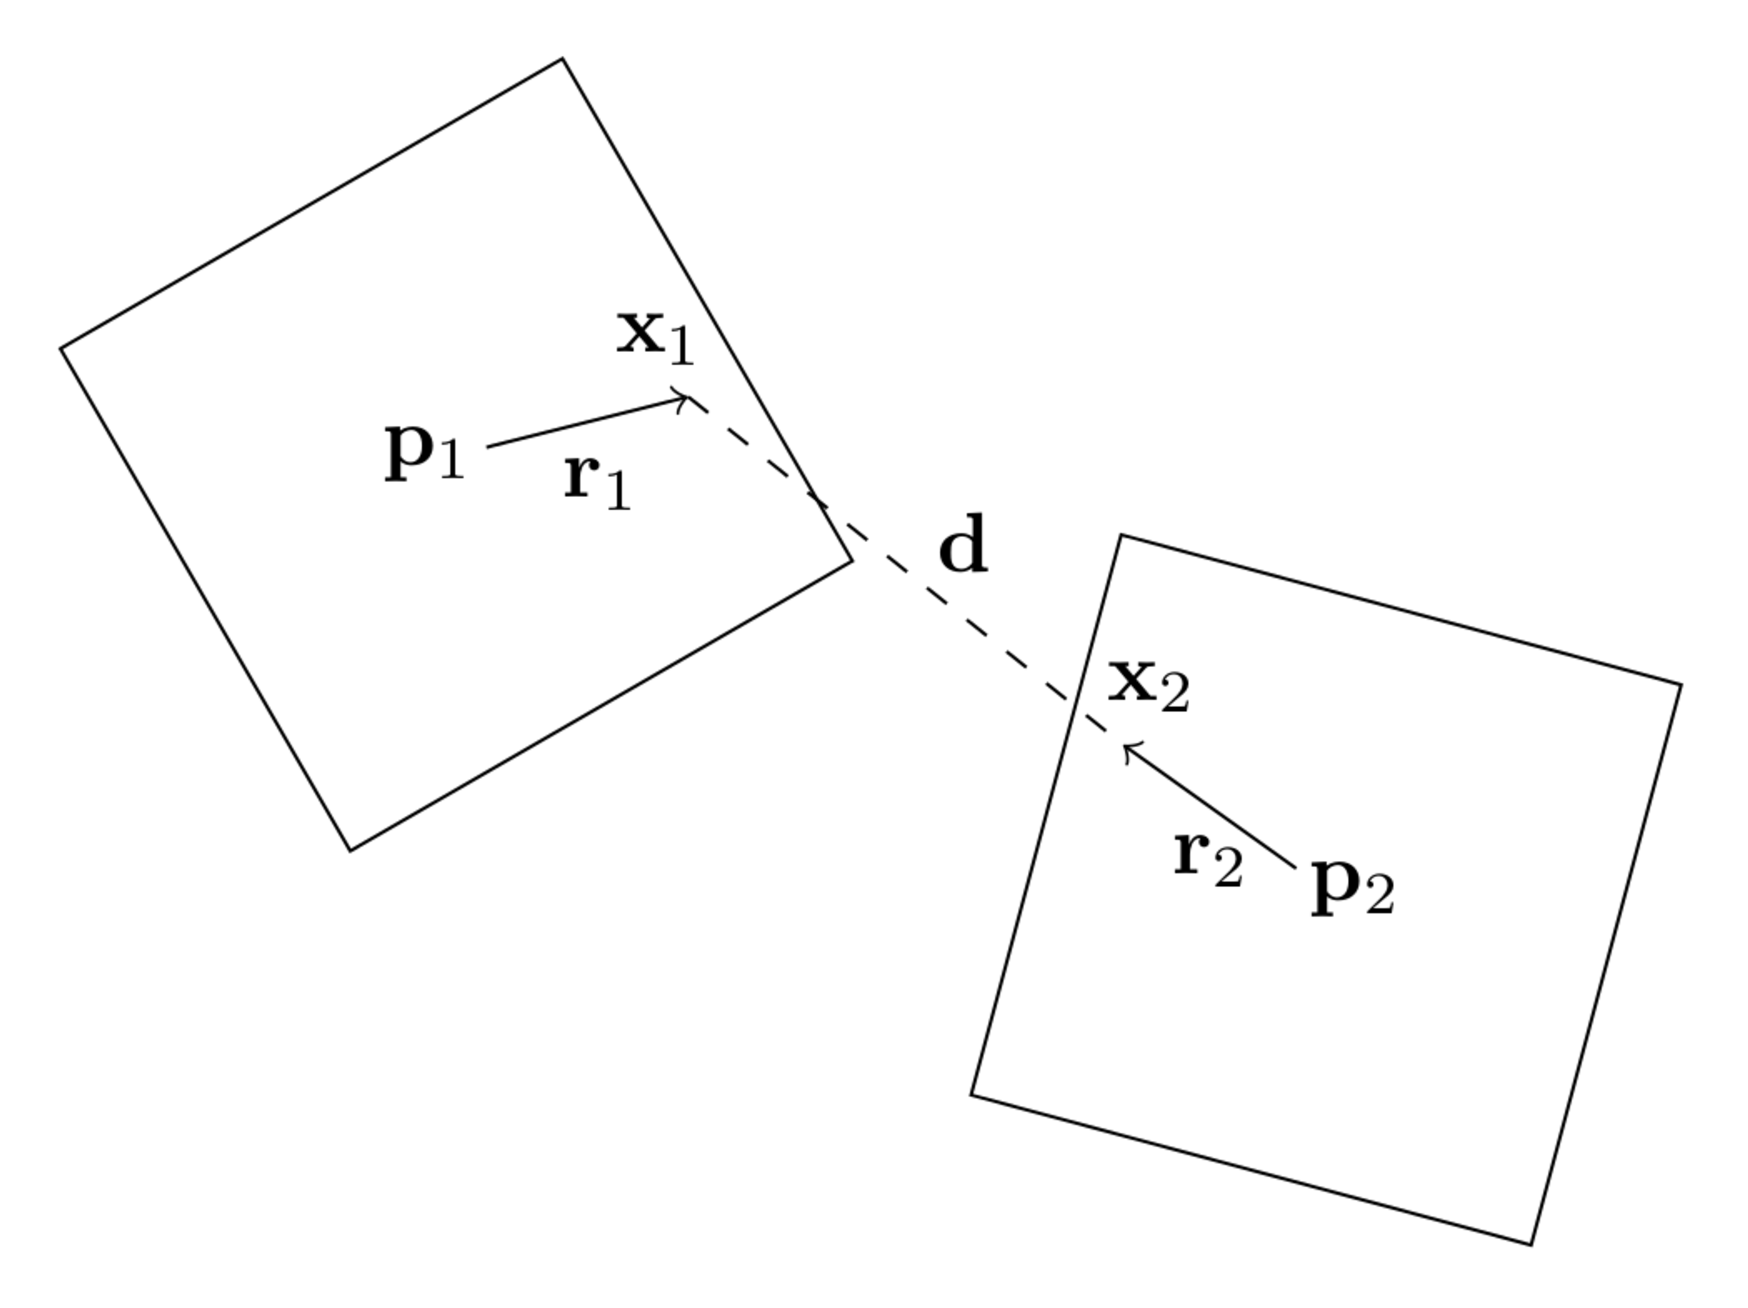
\includegraphics[width=0.35\textwidth]{graphics/constraint_3d_example.eps}
  \caption{3D constraint example}
  \label{fig:constraint_3d_example}
\end{figure}
\FloatBarrier

\begin{itemize}
  \item
    Consider a constraint that keeps points $x_{1}$ and $x_{2}$ a fixed distance
    $L$ apart:
    \[
      C(x_{1}, q_{1}, x_{2}, q_{2}) =
        \frac{1}{2} \left((x_{2} - x_{1})^{2} - L^{2}\right)
    \]

    where $q_{1}$ and $q_{2}$ are orientations of the two cubes.

  \item
    Differentiate $x_{1}$ and $x_{2}$ as vector from position of cube with
    respect to time:
    \begin{align*}
      \frac{dx_{1}}{dt} &= v_{1} + \omega_{1} \times r_{1} \\
      \frac{dx_{2}}{dt} &= v_{2} + \omega_{2} \times r_{2}
    \end{align*}

  \item
    Obtain:
    \[
      \dot C = -d \cdot v_{1} - (r_{1} \times d) \cdot \omega_{1} +
                d \cdot v_{2} + (r_{2} \times d) \cdot \omega_{2}
    \]

  \item
    Gives Jacobian $J$:
    \[
      J = (-d^{T} \quad -(r_{1} \times d)^{T} \quad d^{T} \quad (r_{2} \times d)^{T})
    \]

\end{itemize}

\subsubsection{Adding Energy}

\begin{itemize}
  \item
    Energy is constant when $\dot C = 0$

  \item
    Can set $\dot C$ to a vector function to add or remove energy from the
    system

  \item
    Known as bias vector $\zeta$

    Can relate to position, orientation and time

\end{itemize}

\subsubsection{Constraint Drift and Baumgarte correction}

\begin{itemize}
  \item
    Can introduce a correction factor $\beta$ to deal with accumulated error due
    to iterative updates:
    \[
      \dot C = J V - \beta C
    \]

  \item
    Errors often tied to nature of constraints and time, as such express
    correction as:
    \[
      \dot C(t) + \beta C(t) = 0
    \]

  \item
    $\beta$ is clamped to the range:
    \[
      0 < \beta < \frac{1}{\Delta t}
    \]

\end{itemize}

\subsubsection{Calculating $\lambda$}

\begin{itemize}
  \item
    Force $F$ required to satisfy constraint:
    \[
      F = J^{T} \lambda
    \]

    where $\lambda$ is a constant such that force $F$ balances/solves the
    constraint

  \item
    Need to calculate $\lambda$ for specific objects

  \item
    Consider Newton's second law ($f = ma$):
    \begin{align*}
      F &= M \cdot V \\
      M &= \left[
              \begin{array}{cccc}
                m_{1} & 0     & 0     & 0     \\
                0     & I_{1} & 0     & 0     \\
                0     & 0     & m_{2} & 0     \\
                0     & 0     & 0     & I_{2} \\
              \end{array}
           \right]
    \end{align*}

    Matrix $M$ describes distribution of mass for both objects ($m$ are masses,
    $I$ are inertia tensors) and $\dot V$ is the acceleration equivalent to $V$

  \item
    Approximate $\dot V$ numerically over a small time step $\Delta t$:
    \[
      \dot V \approx \frac{V_{2} - V_{1}}{\Delta t}
    \]

  \item
    Multiply by mass matrix $M$:
    \begin{align*}
      J^{T} \lambda &= M \dot V \\
      J^{T} \lambda &= \frac{M(v_{2} - V_{1})}{\Delta t}
    \end{align*}

  \item
    Multiply by $J M^{-1}$ ($M$ is easily invertible):
    \[
      J M^{-1} J^{T} \lambda = \frac{\zeta - J V}{\Delta t}
    \]

  \item
    Rearrange for $\lambda$:
    \[
      \lambda = \frac{\zeta - J V}{J M^{-1} J^{T} \Delta t}
    \]

\end{itemize}

\subsection{Collision Detection}

\begin{itemize}
  \item
    Performed in two stages:
    \begin{description}
      \item[Broadphase] \hfill
        \begin{itemize}
          \item
            Determine if it is possible for two objects to have collided

          \item
            Reduce the list of collision pairs by excluding those where a
            collision is certainly impossible

          \item
            Computationally fast tests as accuracy is not important at this
            stage

        \end{itemize}

      \item[Narrowphase] \hfill
        \begin{itemize}
          \item
            Determine if two objects have collided

          \item
            Accurate tests

          \item
            Often tests for simple shapes can be used, depending on the
            specifics of the object

            Game object often made up of several simple collision shapes

        \end{itemize}

    \end{description}

  \item
    Collision response data to be extracted from collision detection:
    \begin{description}
      \item[Penetration Depth, $p$] \hfill \\
        Distance the two objects interface/overlap

      \item[Collision Normal, $N$] \hfill \\
        Normal along which the two objects collided

      \item[Contact Point, $P$] \hfill \\
        The point at which the two objects are interfacing

    \end{description}

\end{itemize}

\subsubsection{Broadphase: Bounding volume test}

\begin{itemize}
  \item
    Simplest (but effective) test

  \item
    Test for intersection of bounding volumes

  \item
    Typically either sphere or axis aligned bounding box due to efficiency of
    test

\end{itemize}

\subsubsection{Broadphase: World Partitioning}

\begin{itemize}
  \item
    Split world into partitions and only test for collision between objects in
    the same partition

  \item
    Objects may reside in multiple partitions (if they are on the border of
    several partitions)

  \item
    Common techniques are:
    \begin{description}
      \item[Fixed World Partitioning] \hfill
        \begin{itemize}
          \item
            World is split into predetermined partitions

          \item
            Efficiency over brute force broadphase dependant on distribution of
            objects

        \end{itemize}

      \item[Binary Search Partitioning] \hfill
        \begin{itemize}
          \item
            Recursively partition the world

          \item
            Continue to split the world until either a maximum depth or number
            of objects in a division is reached

          \item
            Distributes partitions according to object distribution so maintains
            efficiency regardless of world state

          \item
            Octree and quadtree are common implementations, dividing each
            partition into 8 or 4 sub-partitions respectively

        \end{itemize}

    \end{description}

\end{itemize}

\subsubsection{Broadphase: Sort and Sweep}

\begin{itemize}
  \item
    Project bounding volumes onto a single axis and create possible collision
    pairs from overlapping volumes

  \item
    Workflow:
    \begin{enumerate}
      \item[1]
        Sort objects based on their position along the sort axis

      \item[2]
        Traverse the list, when the start of object $O_{i}$ is found and other
        objects that are encountered before the end of $O_{i}$ are potential
        collision pairs

    \end{enumerate}

\end{itemize}

\subsubsection{Narrowphase: Separating Axis Theorem (SAT)}

\begin{itemize}
  \item
    If two objects are not interfacing then it should be possible to draw a
    plane between them

  \item
    Only works for convex shapes

  \item
    If a single can where a plane can be drawn between two objects then the two
    objects are certainly not interfacing

  \item
    Test by projecting the shapes onto a test axis and checking for overlap
    between them

\end{itemize}

\begin{figure}[h!]
  \centering
  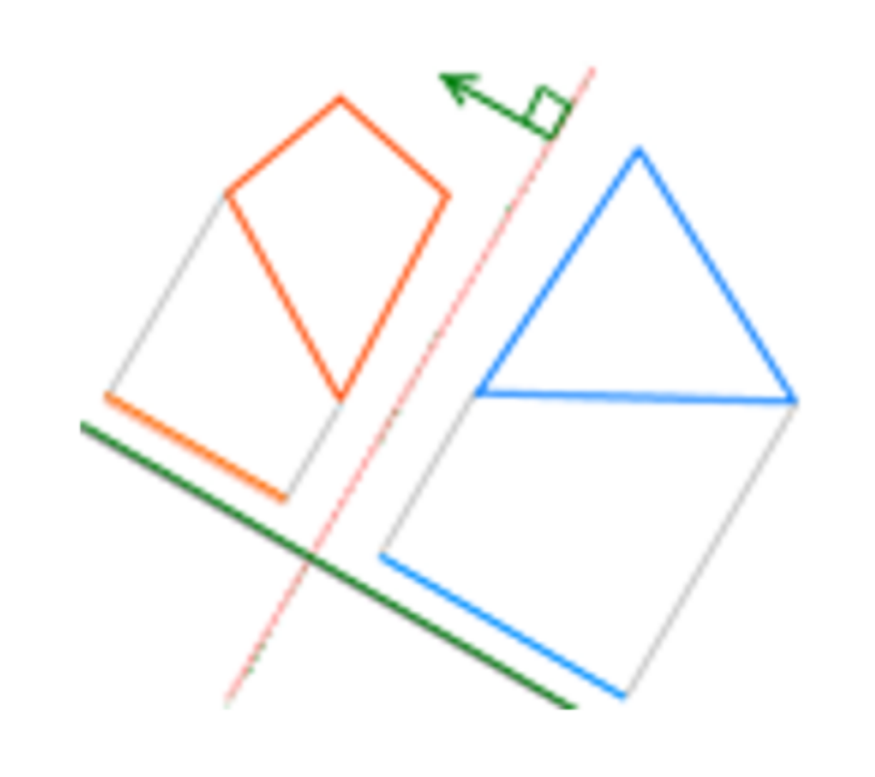
\includegraphics[width=0.25\textwidth]{graphics/coll_det_sat.eps}
  \caption{SAT collision detection}
  \label{fig:coll_det_sat}
\end{figure}
\FloatBarrier

\Para{Generating potential separating axes}

\begin{itemize}
  \item
    Assuming only polygonal shapes the potential collision axes are defined by
    the normals of each face of the collision shapes

  \item
    Number of potential separating axis is the number of faces of each shape
    combined

  \item
    As soon as a single separating axis is found in which the projections of the
    objects do not overlap the algorithm can exit (without having to test all
    axes)

  \item
    Parallel axis do not need to be checked multiple times

\end{itemize}

\begin{figure}[h!]
  \centering
  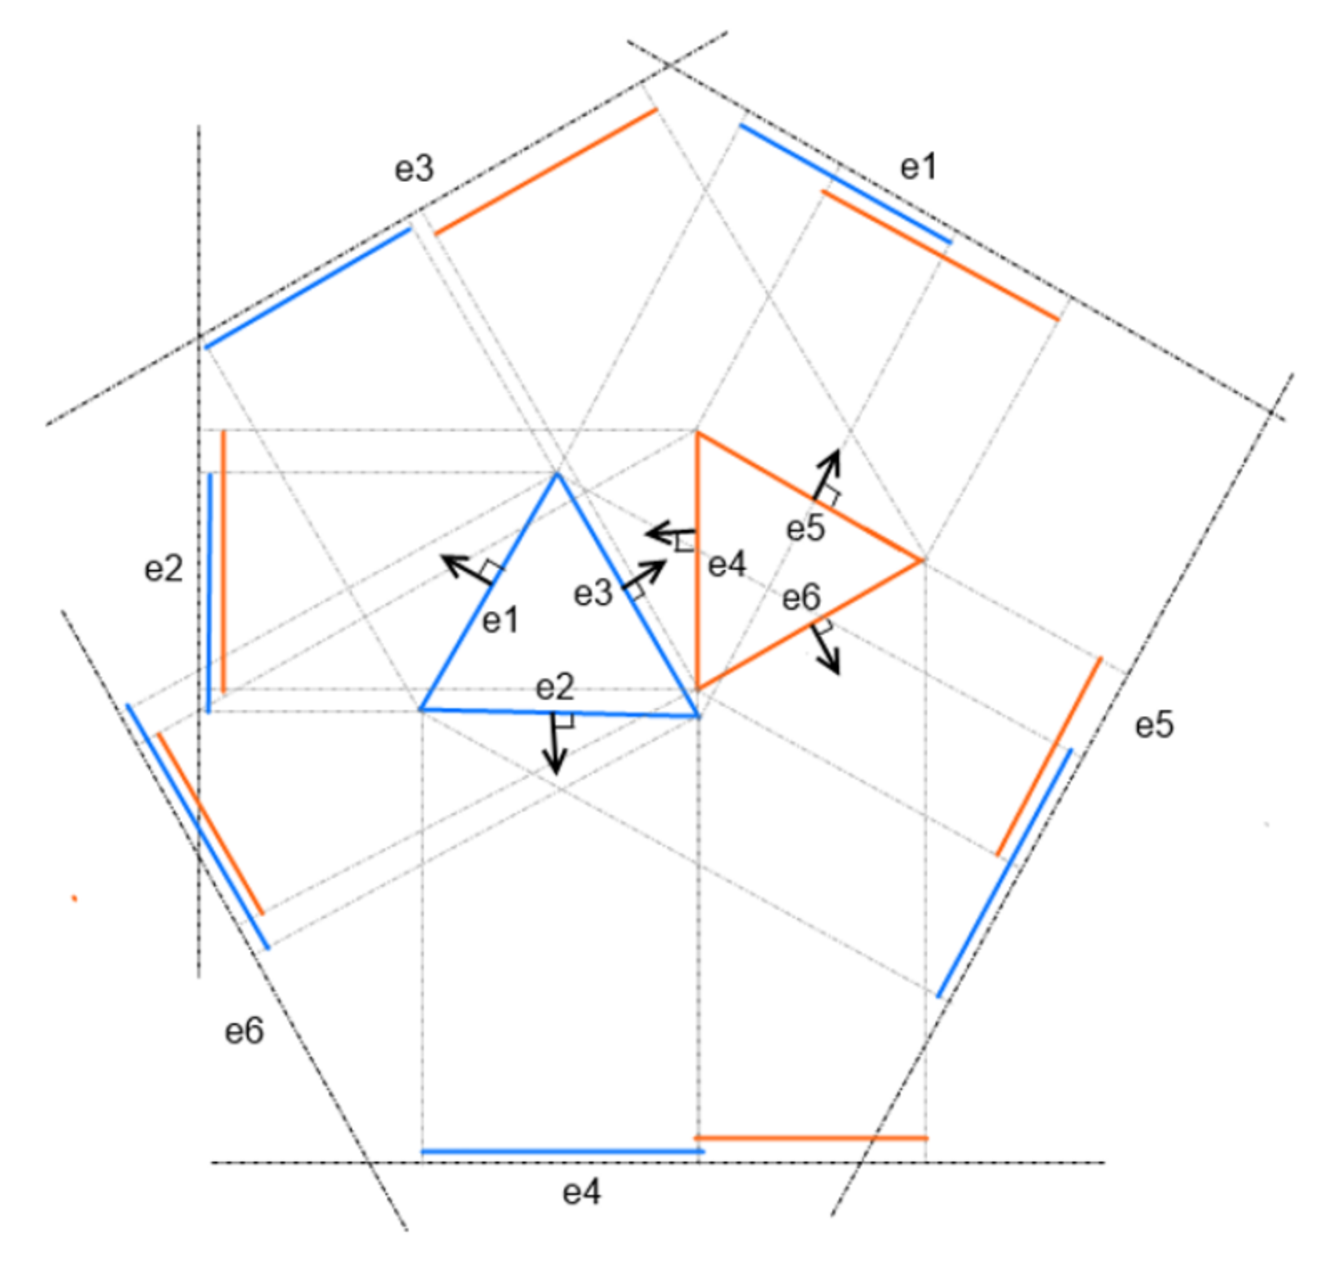
\includegraphics[width=0.5\textwidth]{graphics/coll_det_sat_axes.eps}
  \caption{SAT potential collision axes}
  \label{fig:coll_det_sat_axes}
\end{figure}
\FloatBarrier

\Para{Edge-Edge collisions in 3D}

\begin{itemize}
  \item
    Figure \ref{fig:colldet_sat_3d} shows a case where SAT generates a false
    positive when two 3D objects are not actually colliding but all potential
    axis tests show them to be overlapping

  \item
    Generate additional potential separating axis using the cross product of
    every permutation of faces on both object

  \item
    Creates a set of new potential separating axes which are orthogonal to pairs
    of faces

  \item
    Vast increase in number of potential separating axes

\end{itemize}

\begin{figure}[h]
  \centering

  \begin{subfigure}[b]{0.3\textwidth}
    \centering
    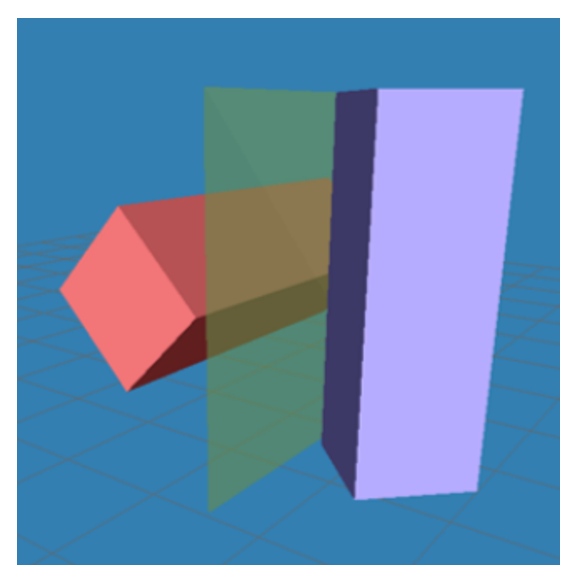
\includegraphics[width=0.8\textwidth]{graphics/colldet_sat_3d_1.eps}
  \end{subfigure}
  \begin{subfigure}[b]{0.3\textwidth}
    \centering
    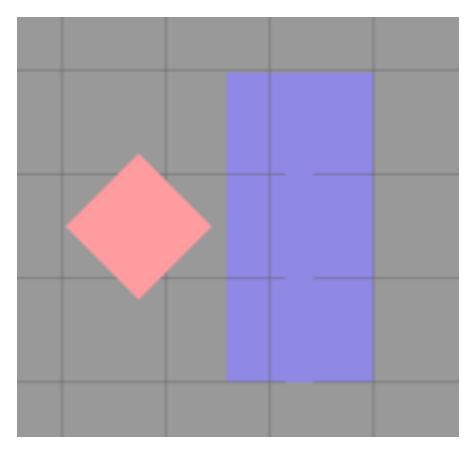
\includegraphics[width=0.8\textwidth]{graphics/colldet_sat_3d_2.eps}
  \end{subfigure}

  \vspace{1em}

  \begin{subfigure}[b]{0.32\textwidth}
    \centering
    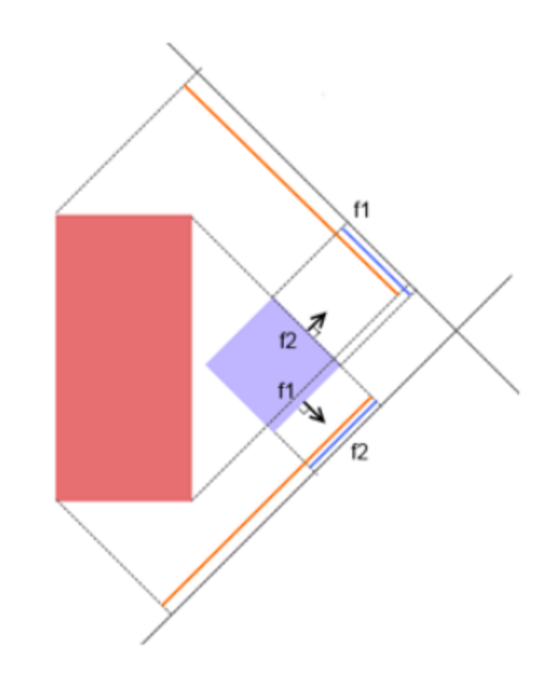
\includegraphics[width=0.6\textwidth]{graphics/colldet_sat_3d_top.eps}
    \caption{Top ($-y$)}
  \end{subfigure}
  \begin{subfigure}[b]{0.32\textwidth}
    \centering
    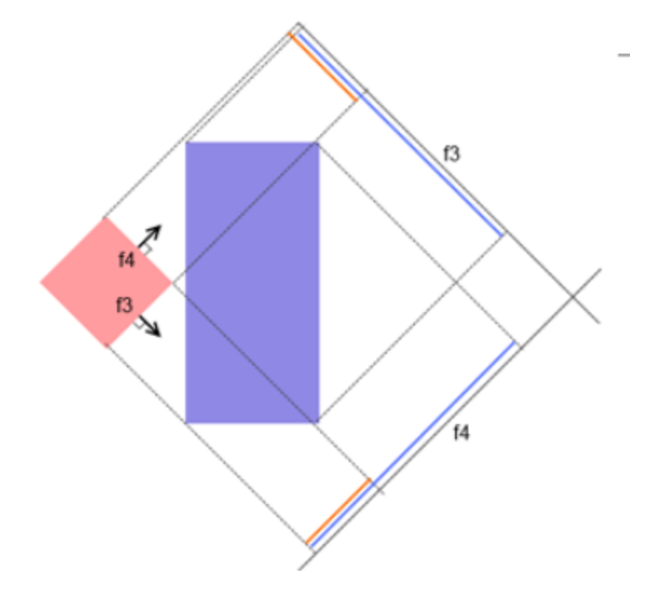
\includegraphics[width=0.8\textwidth]{graphics/colldet_sat_3d_front.eps}
    \caption{Front ($-z$)}
  \end{subfigure}
  \begin{subfigure}[b]{0.32\textwidth}
    \centering
    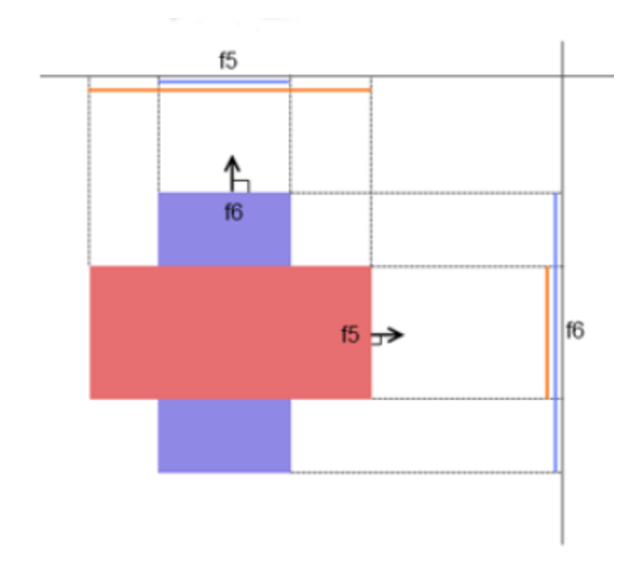
\includegraphics[width=0.8\textwidth]{graphics/colldet_sat_3d_left.eps}
    \caption{Left ($+x$)}
  \end{subfigure}

  \caption{SAT in 3D}
  \label{fig:colldet_sat_3d}
\end{figure}
\FloatBarrier

\Para{Spheres and Curves}

\begin{itemize}
  \item
    Curves have an infinite number of edges

  \item
    As shapes are convex only one axis must be tested to check if shapes are
    colliding

  \item
    For sphere-sphere simply test the distance between the closest point of
    object 1 with the closest point of object 2

  \item
    For sphere-polygon iterate through all faces of the polygon to find the face
    on which the closest point to the sphere resides, the normal of this face is
    the potential separating axis

\end{itemize}

\begin{figure}[h]
  \centering

  \begin{subfigure}[b]{0.4\textwidth}
    \centering
    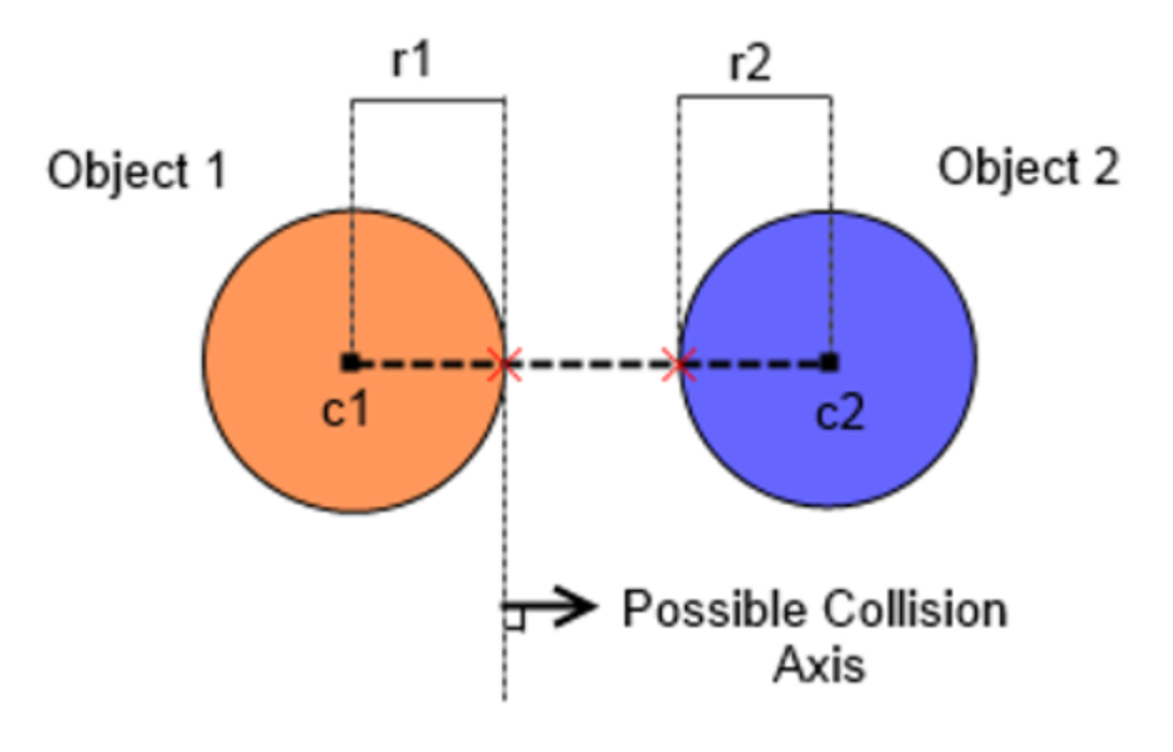
\includegraphics[width=0.8\textwidth]{graphics/colldet_sat_sphere_sphere.eps}
    \caption{Sphere-Sphere}
  \end{subfigure}
  \begin{subfigure}[b]{0.3\textwidth}
    \centering
    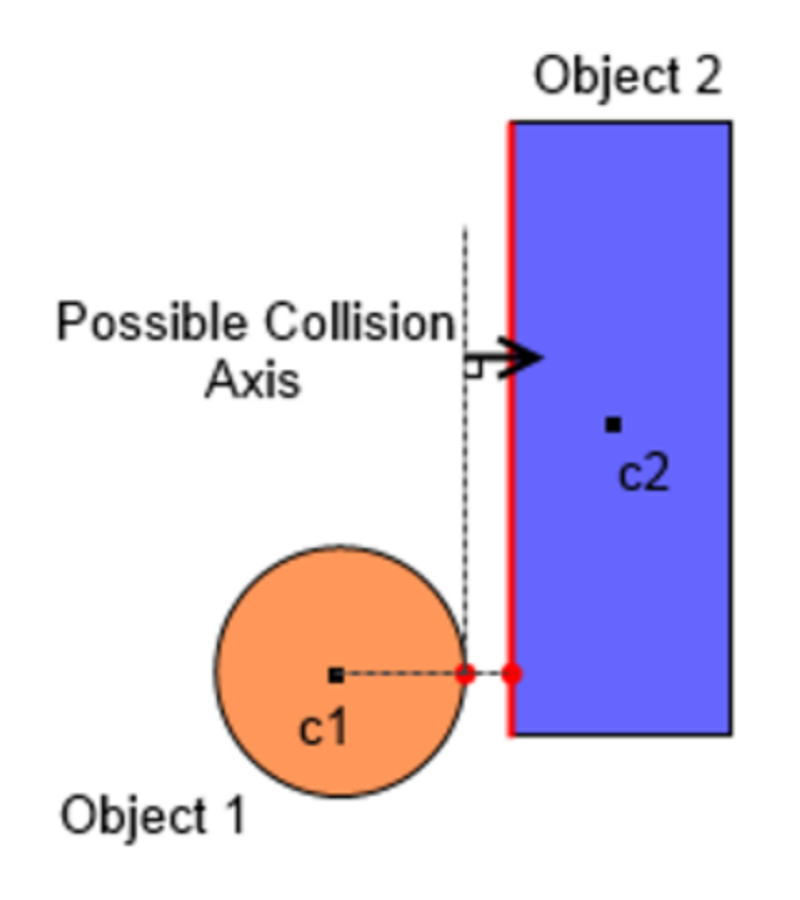
\includegraphics[width=0.8\textwidth]{graphics/colldet_sat_sphere_polygon.eps}
    \caption{Sphere-Polygon}
  \end{subfigure}

  \label{fig:colldet_sat_curves}
\end{figure}
\FloatBarrier

\subsubsection{Sphere-Sphere test}

\begin{itemize}
  \item
    Two spheres of radii $r_{1}$ and $r_{2}$ at positions $S_{1}$ and $S_{2}$
    have collided if:
    \begin{align*}
      d &< r_{1} + r_{2} \\
      d &= \sqrt{(x_{2} - x_{1})^{2} + (y_{2} - y_{1})^{2} + (z_{2} - z_{1})^{2}}
    \end{align*}
    where $d$ is the distance between the circle centres.

  \item
    For computational savings can be simplified to:
    \begin{align*}
      d^{2} &< (r_{1} + r_{2})^{2} \\
      d^{2} &= (x_{2} - x_{1})^{2} + (y_{2} - y_{1})^{2} + (z_{2} - z_{1})^{2}
    \end{align*}

  \item
    Collision response data:
    \begin{align*}
      p &= r_{1} + r_{2} - d \\
      N &= |S_{1} - S_{2}| \\
      P &= S_{1} - N(r_{1} - p)
    \end{align*}

\end{itemize}

\subsubsection{AABB-AABB test}

\begin{itemize}
  \item
    Two AABB of dimensions $(w_{1}, h_{1}, l_{1})$ and $(w_{2}, h_{2}, l_{2})$
    at positions $(x_{1}, y_{1}, l_{2})$ and $(x_{2}, y_{2}, z_{2})$ are
    interfacing the three conditions are all true:
    \begin{align*}
      |x_{2} - x_{1}| &< \frac{1}{2}(w_{1} + w_{2}) \\
      |y_{2} - y_{1}| &< \frac{1}{2}(h_{1} + h_{2}) \\
      |z_{2} - z_{1}| &< \frac{1}{2}(l_{1} + l_{2})
    \end{align*}

  \item
    Computationally cheap, but limited as bounding boxes must be axis aligned

\end{itemize}

\subsubsection{Sphere-Plane test}

\begin{itemize}
  \item
    Sphere at position $S$ of radius $r$ intersects an infinite plane with
    normal $N$ at distance $d$ from the origin if:
    \[
      N \cdot S -d < r
    \]

  \item
    Collision response data:
    \begin{align*}
      p &= r - (N \cdot S - d) \\
      N &= N_{plane} \\
      P &= S - N(r - p)
    \end{align*}

\end{itemize}

\begin{figure}[h!]
  \centering
  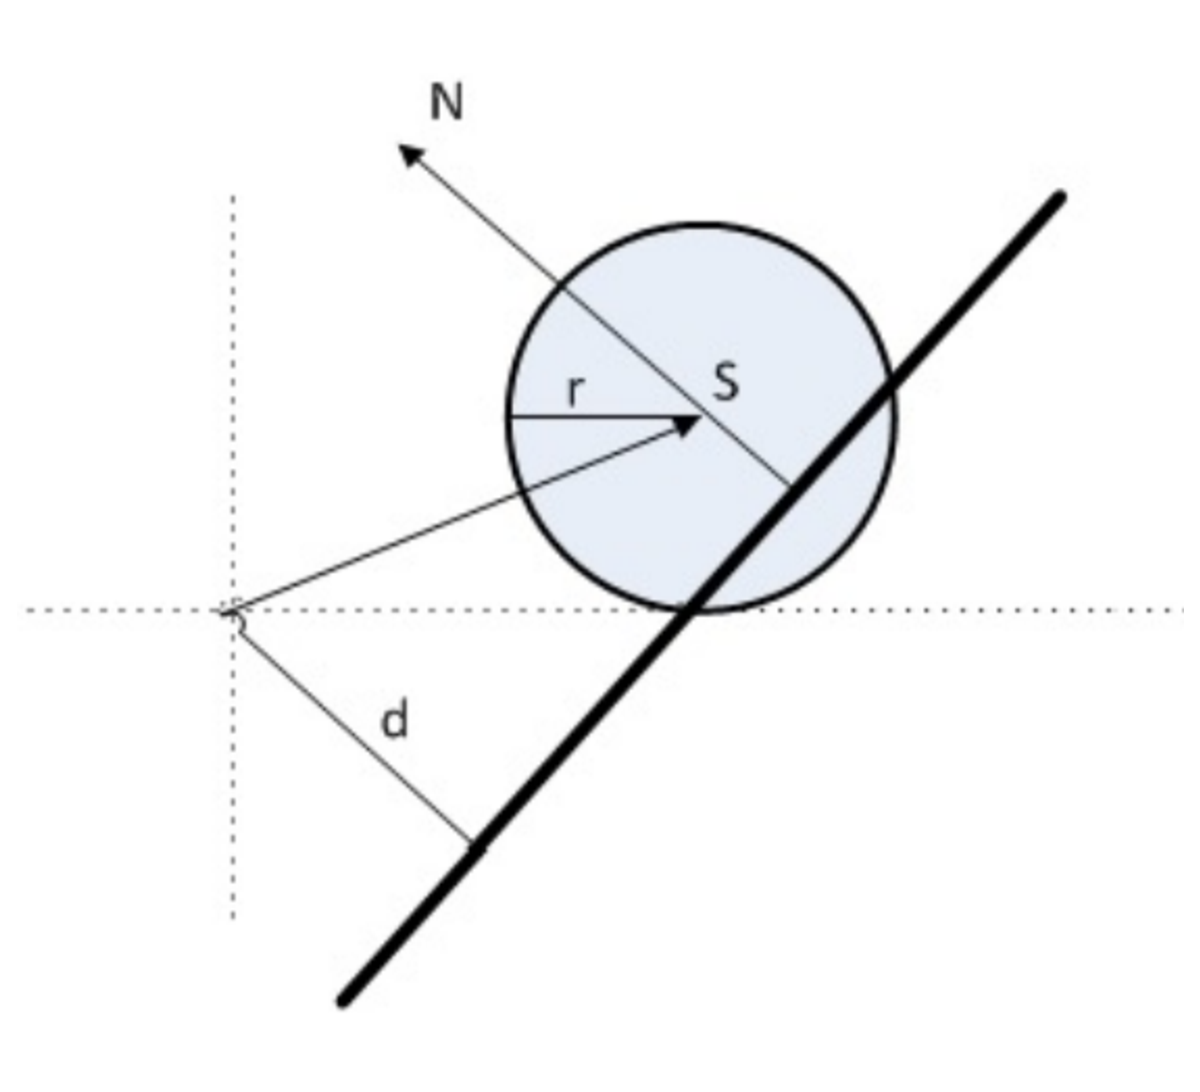
\includegraphics[width=0.3\textwidth]{graphics/plane_collision_detection.eps}
  \caption{Sphere-Plane collision test}
  \label{fig:plane_collision_detection}
\end{figure}
\FloatBarrier

\subsection{Collision Manifolds}

\begin{itemize}
  \item
    Specify multiple points of contact for an interface rather than just one

  \item
    Summation of surface area between two colliding objects

  \item
    Manifold is created as a 2D surface, even though by the time a collision has
    been detected there will be an intersecting volume between the two object

\end{itemize}

\subsubsection{Clipping method}

\begin{itemize}
  \item
    Obtain a manifold that describes the initial collision points accurately

  \item
    Omit any contact points that are a result of collisions after the objects
    intersect each other

  \item
    With convex object typically there will be only one or two contact points

\end{itemize}

\Para{Worked example}

\begin{itemize}
  \item
    Using hypothetical collision shown in figure \ref{fig:manifolds_clipping_0}

  \item
    Have collision normal and penetration depth from SAT

\end{itemize}

\begin{figure}[h!]
  \centering
  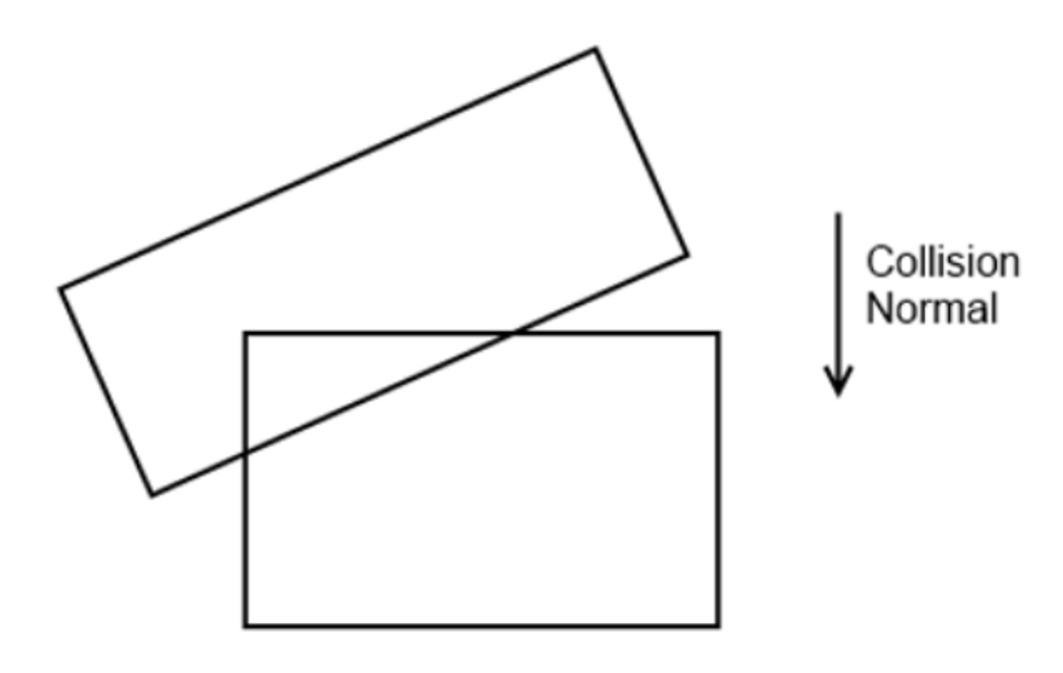
\includegraphics[width=0.35\textwidth]{graphics/manifolds_clipping_0.eps}
  \caption{Example collision}
  \label{fig:manifolds_clipping_0}
\end{figure}
\FloatBarrier

Workflow:
\begin{enumerate}
  \item[1]
    Identify Significant Faces
    \begin{itemize}
      \item
        Identify the two significant faces that are intersecting

      \item
        For each shape:
        \begin{itemize}
          \item
            Select the vertex furthest along the collision normal (shown in red
            in figure \ref{fig:manifolds_clipping_1})

          \item
            Select the face that includes this vertex that has a normal closest
            to the collision normal

        \end{itemize}

      \item
        The faces selected for both shapes are the significant faces

    \end{itemize}

    \begin{figure}[h!]
      \centering
      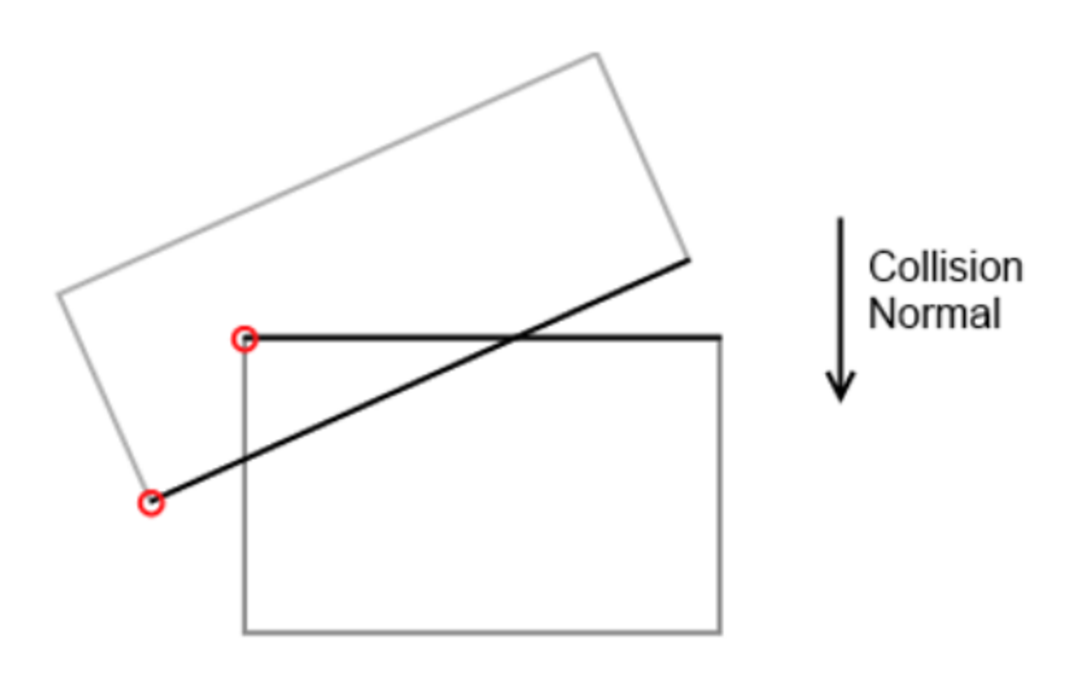
\includegraphics[width=0.35\textwidth]{graphics/manifolds_clipping_1.eps}
      \caption{Significant faces}
      \label{fig:manifolds_clipping_1}
    \end{figure}
    \FloatBarrier

  \item[2]
    Determining Incident and Reference Faces
    \begin{itemize}
      \item
        The reference face will be the point of reference when clipping

      \item
        The incident face will be the set of vertices being clipped

      \item
        The face with a normal closest to the collision normal becomes the
        reference face

        The other face is the incident face

    \end{itemize}

    \begin{figure}[h!]
      \centering
      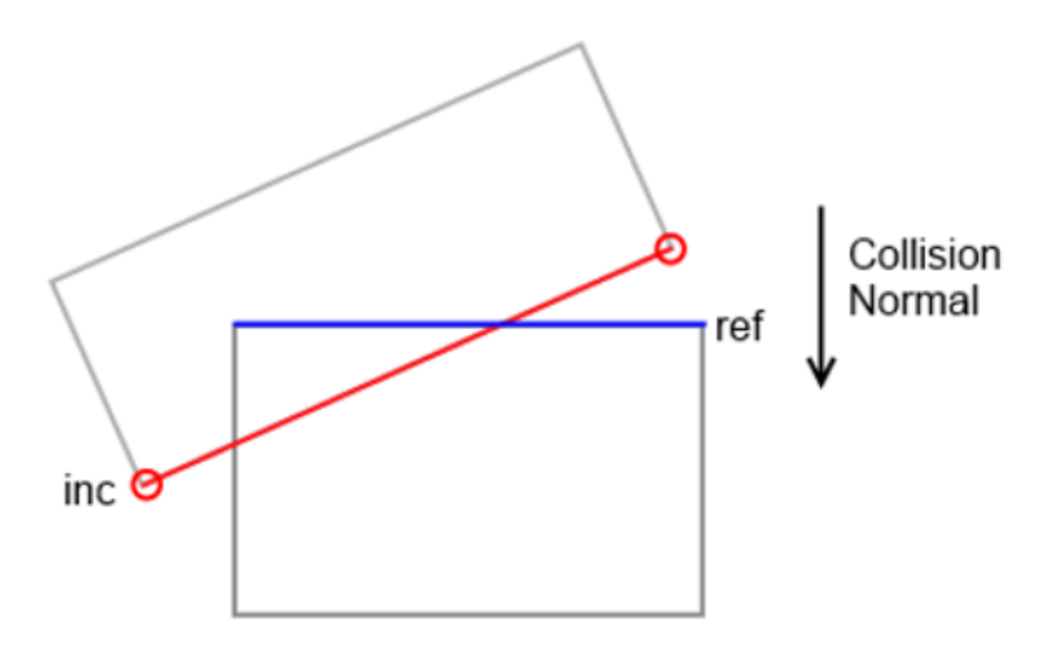
\includegraphics[width=0.35\textwidth]{graphics/manifolds_clipping_2.eps}
      \caption{Incident and Reference faces}
      \label{fig:manifolds_clipping_2}
    \end{figure}
    \FloatBarrier

  \item[3]
    Adjacent face clipping
    \begin{itemize}
      \item
        Clip the incident face with all adjacent face of the reference face

      \item
        Using the normal of adjacent faces and any vertex on the face to produce
        a plane equation

      \item
        Use Sutherland-Hodgman Clipping algorithm

      \item
        Clipped edges will have new vertices added as shown on the left hand
        side in figure \ref{fig:manifolds_clipping_3}

    \end{itemize}

    \begin{figure}[h!]
      \centering
      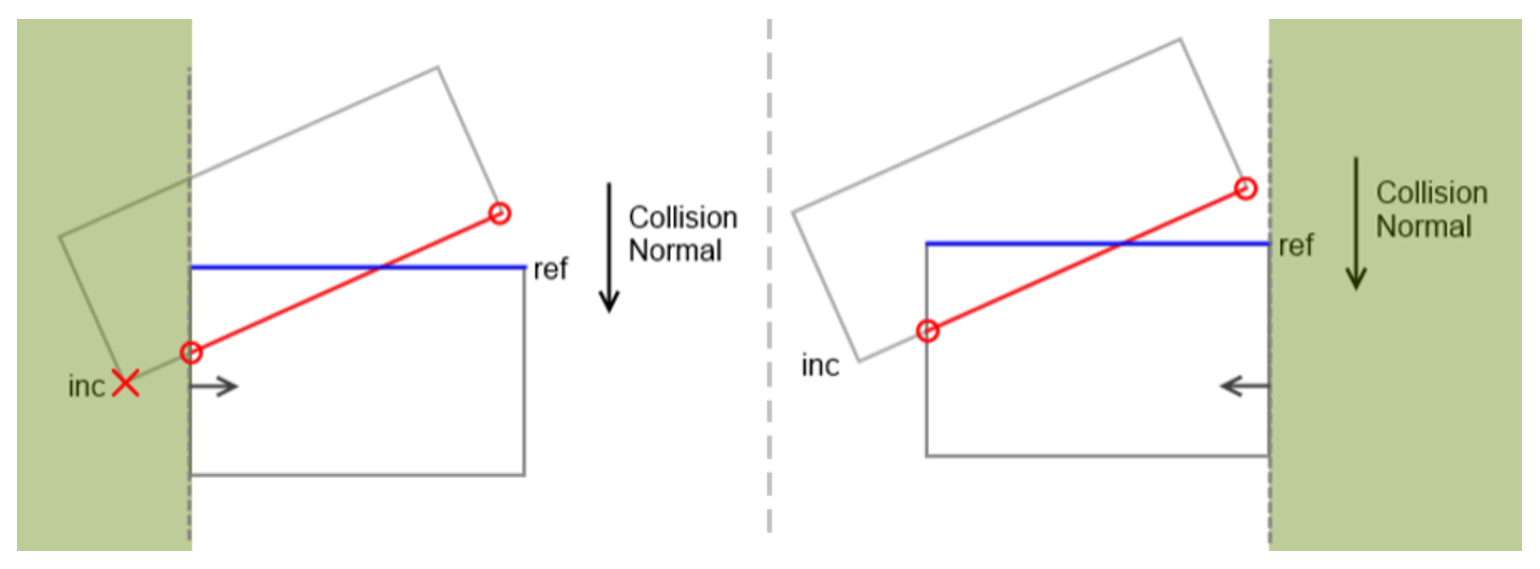
\includegraphics[width=0.7\textwidth]{graphics/manifolds_clipping_3.eps}
      \caption{Adjacent face clipping (clipping region shaded green)}
      \label{fig:manifolds_clipping_3}
    \end{figure}
    \FloatBarrier

  \item[4]
    Final clipping
    \begin{itemize}
      \item
        Final clipping is in the plane of the reference face

      \item
        Remove all points in clipping plane (as opposed to non-destructive
        clipping in previous stage)

      \item
        This leaves the original collision points and removes any that occur
        after the two objects intersect each other

    \end{itemize}

    \begin{figure}[h!]
      \centering
      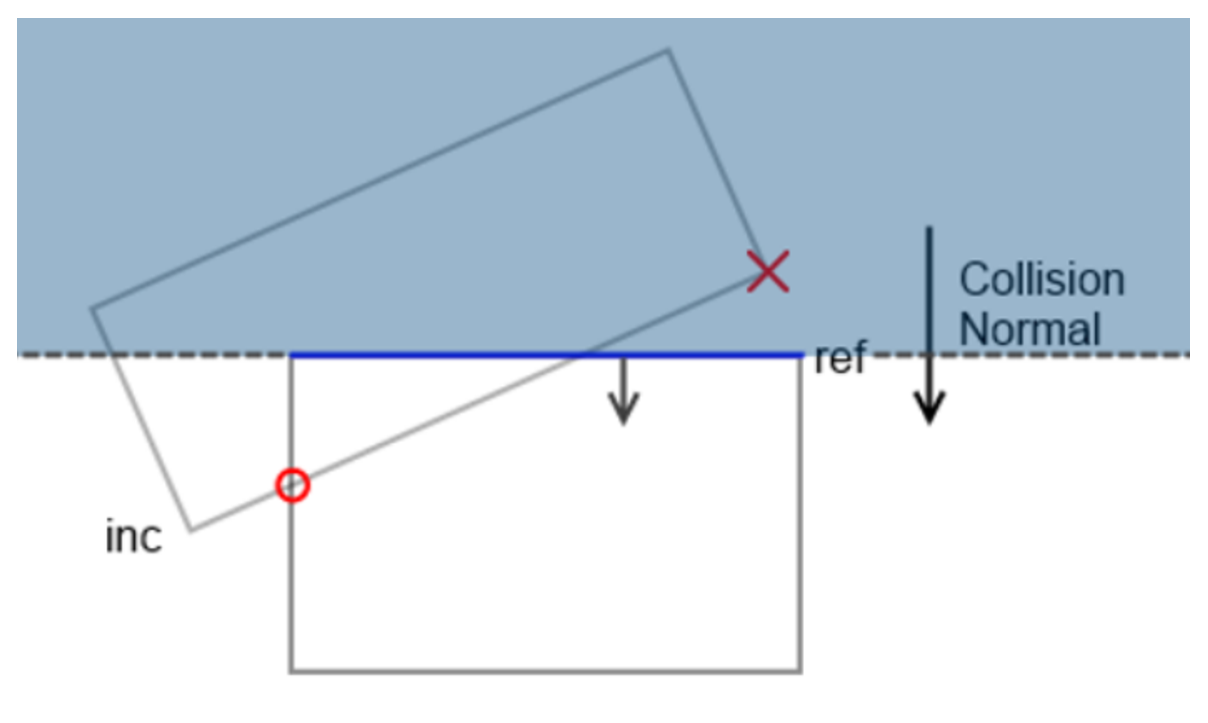
\includegraphics[width=0.4\textwidth]{graphics/manifolds_clipping_4.eps}
      \caption{Final clipping (clipping region shaded blue)}
      \label{fig:manifolds_clipping_4}
    \end{figure}
    \FloatBarrier

\end{enumerate}

\subsection{Collision Response}

\begin{itemize}
  \item
    Resolve collisions using:
    \begin{itemize}
      \item
        The collision manifold

      \item
        The collision normal

      \item
        The penetration depth

    \end{itemize}

  \item
    General methods of collision response:
    \begin{description}
      \item[Projection methods] \hfill \\
        Control the position of colliding objects

      \item[Impulse methods] \hfill \\
        Control the velocity of colliding objects

      \item[Penalty methods] \hfill \\
        Control the acceleration of colliding objects

    \end{description}

\end{itemize}

\subsubsection{Impulse method}

\begin{itemize}
  \item
    Apply an impulse $J$ to each object:
    \begin{align*}
      J &= F \Delta t \\
        &= ma \Delta t \\
        &= m \frac{\Delta v}{\Delta t} \Delta t \\
        &= m \Delta v
    \end{align*}

  \item
    Affect velocity of each object using impulse:
    \[
      \Delta v = \frac{J}{m}
    \]

\end{itemize}

\Para{Linear impulse}

\begin{itemize}
  \item
    Calculate relative velocity of colliding entities along collision normal:
    \begin{align*}
      v_{ab} &= v_{a} - v_{b} \\
      v_{n} &= v_{ab} \cdot N
    \end{align*}

  \item
    Final relative velocity dependant on coefficient of elasticity $\epsilon$
    \begin{itemize}
      \item
        $\epsilon = 1$ is a purely elastic collision (no loss of velocity in
        collision)

      \item
        $\epsilon = 0$ is a purely inelastic collision (no velocity transfer,
        objects stick together)

    \end{itemize}

  \item
    Impulse calculated as:
    \[
      J = \frac{-(1 + \epsilon) v_{ab} \cdot N}
               {N \cdot N\left(\frac{1}{m_{a}} + \frac{1}{m_{b}}\right)}
    \]

  \item
    Ensure conservation of momentum plus impulse to resolve collision:
    \begin{align*}
      m_{a}v_{a}^{f} &= m_{a}v_{a}^{i} + J N \\
      m_{b}v_{b}^{f} &= m_{b}v_{b}^{i} + J N
    \end{align*}

  \item
    Velocity updates:
    \begin{align*}
      v_{a}^{f} &= v_{a}^{i} + \frac{J}{m_{a}} N \\
      v_{b}^{f} &= v_{b}^{i} + \frac{J}{m_{b}} N
    \end{align*}

\end{itemize}

\Para{Angular impulse}

\begin{itemize}
  \item
    Need to take into account velocity of contact points due to angular
    velocity:
    \begin{align*}
      v_{ca} &= v_{a} \hl{+ \omega_{a} r_{a}} \\
      v_{cb} &= v_{b} \hl{+ \omega_{b} r_{b}}
    \end{align*}

  \item
    Addition to impulse calculation:
    \[
      J = \frac{-(1 + \epsilon) v_{ab} \cdot N}
               {N \cdot N\left(\frac{1}{m_{a}} + \frac{1}{m_{b}}\right)
                \hl{+ \left[
                      \left(I_{a}^{-1} \left(r_{b} \times N\right)\right) \times r_{a} +
                      \left(I_{b}^{-1} \left(r_{b} \times N\right)\right) \times r_{b}
                      \right] \cdot N
                   }
               }
    \]

  \item
    Ensure conservation of momentum:
    \begin{align*}
      I_{a} \omega_{a}^{f} &= I_{a} \omega_{a}^{i} + r_{a} \times J N \\
      I_{b} \omega_{b}^{f} &= I_{b} \omega_{b}^{i} + r_{b} \times J N
    \end{align*}

  \item
    Angular velocity updates:
    \begin{align*}
      \omega_{a}^{f} &= \omega_{a}^{i} + \frac{r_{a} \times J N}{I_{a}} \\
      \omega_{b}^{f} &= \omega_{b}^{i} - \frac{r_{b} \times J N}{I_{b}} \\
    \end{align*}

\end{itemize}

\subsubsection{Penalty method}

\begin{itemize}
  \item
    Model collision as a spring

  \item
    Spring equation with damping:
    \[
      F = -kx - cv
    \]

    $F$ is the force extorted by the spring

    $k$ is the spring constant

    $x$ is the displacement of the spring from it s rest position

    $c$ is the damping coefficient

    $v$ is the velocity of the moving object attached to the spring

  \item
    Calculate force for collision:
    \begin{align*}
      F &= -kx - c(N \cdot V_{ab}) \\
      F &= ma \\
    \end{align*}

  \item
    Calculate acceleration of each object:
    \begin{align*}
      a_{1} &= \frac{F}{m_{1}} \\
      a_{2} &= \frac{F}{m_{2}}
    \end{align*}

\end{itemize}

\subsubsection{Soft Bodies}

\begin{itemize}
  \item
    Represent soft bodies as a mesh of nodes connected by springs

  \item
    Commonly use the graphical mesh as the node mesh

  \item
    Expensive to simulate

  \item
    Cannot usually use springs to model deformable objects where the object is
    permanently deformed

    (possible depending on situation, e.g. cloth can be torn by simply removing
    constraints then splitting and filling in the graphical mesh)

\end{itemize}

\subsubsection{Constraint based collision response}

\begin{figure}[h!]
  \centering
  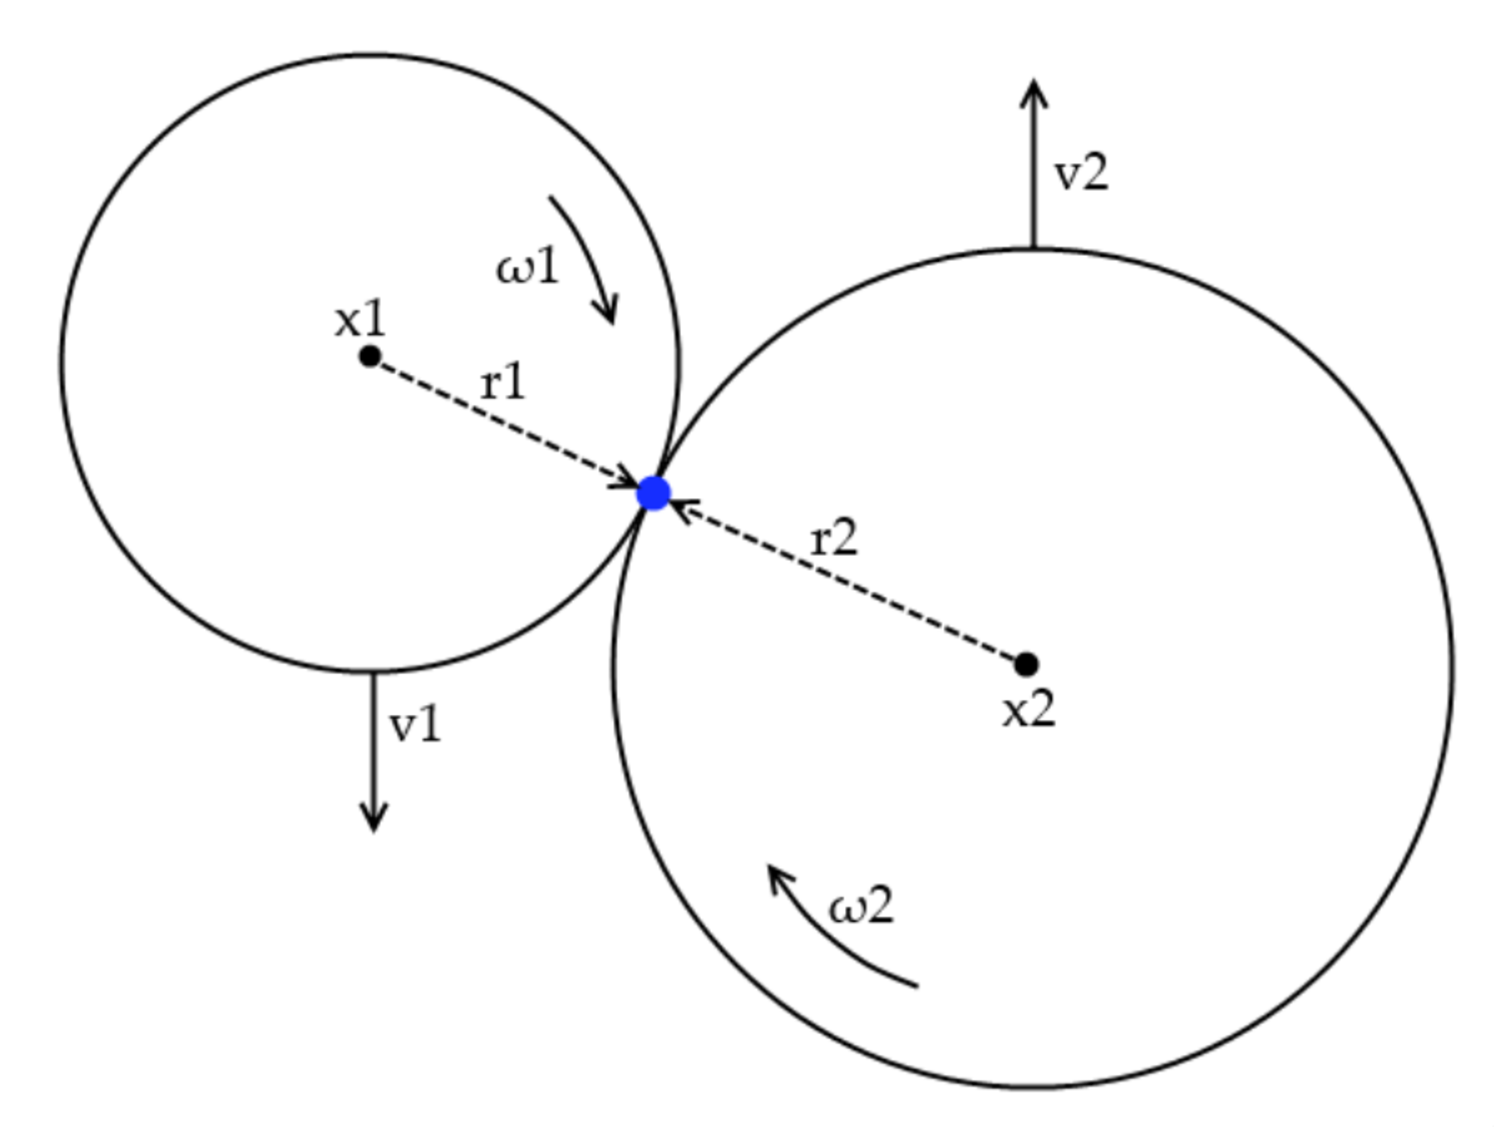
\includegraphics[width=0.4\textwidth]{graphics/collision_constraint_example.eps}
  \caption{Collision constraint example}
  \label{fig:collision_constraint_example}
\end{figure}
\FloatBarrier

\begin{itemize}
  \item
    Inequality restraints restrict the axis, direction, area, etc. in which a
    constraint can act

    Do this by clamping $\lambda$:
    \[
      \lambda_{-} \leq \lambda \leq \lambda_{+}
    \]

  \item
    Contact constraint only allows constraint force to push out (does not affect
    other constraints)

    \begin{align*}
      \lambda_{-} &= 0 \\
      \lambda_{+} &= \infty
    \end{align*}

  \item
    Collision constraint:
    \[
      C = (x_{x} + r_{2} - x_{1} - r_{1}) \cdot N
    \]

  \item
    Contact point $p$ is defined as:
    \[
      p = x + r
    \]

  \item
    Obtain Jacobian:
    \[
      J = \left[
            \begin{array}{c}
              -N^{T}                \\
              -(r_{1} \times N)^{T} \\
              N^{T}                 \\
              (r_{2} \times N)^{T}  \\
            \end{array}
          \right]
    \]

  \item
    Collision is resolved by solving this constraint with the contact constraint
    on $\lambda$

  \item
    Two options for using the collision manifold:
    \begin{enumerate}
      \item[1]
        \begin{itemize}
          \item
            Iterate through all contact points in manifold

          \item
            Majority of collision resolved by first point, majority of remainder
            by second point, etc.

          \item
            Slight loss of accuracy

        \end{itemize}

      \item[2]
        \begin{itemize}
          \item
            Divide the constraint resolution between contact points

        \end{itemize}
    \end{enumerate}

\end{itemize}

\subsubsection{Constraints as Friction}

\begin{itemize}
  \item
    Define tangents to surfaces that are in contact $u_{1}$ and $u_{2}$ and
    their normal $n$:
    \[
      u_{1} \times u_{2} = n
    \]

  \item
    Define collision constraints:
    \begin{align*}
      C_{1} &= (x_{2} + r_{2} - x_{1} - r_{1}) \cdot u_{1} \\
      C_{2} &= (x_{2} + r_{2} - x_{1} - r_{1}) \cdot u_{2}
    \end{align*}

  \item
    Constraints restrict movement of the contact points alone the surface in any
    direction

  \item
    Obtain Jacobians:
    \begin{align*}
      J_{1} = \left[
                \begin{array}{c}
                  -u_{1}^{T}                \\
                  -(r_{1} \times u_{1})^{T} \\
                  u_{1}^{T}                 \\
                  (r_{2} \times u_{1})^{T}  \\
                \end{array}
              \right]
      J_{2} = \left[
                \begin{array}{c}
                  -u_{2}^{T}                \\
                  -(r_{1} \times u_{2})^{T} \\
                  u_{2}^{T}                 \\
                  (r_{2} \times u_{2})^{T}  \\
                \end{array}
              \right]
    \end{align*}

  \item
    Approximate limits on $\lambda$ based on frictional force due to gravity:
    \[
      -\mu m g \leq \lambda \leq \mu m g
    \]

    where $m$ is object mass, $g$ is acceleration due to gravity and $\mu$ is a
    constant which is tuned to make the constraint believable

\end{itemize}

\subsection{Solvers}

\begin{itemize}
  \item
    As more constraints are added to a physics system the need to solve all
    constraints simultaneously arises

  \item
    Objects may be affected by multiple constraints which may work against each
    other if solving constraints sequentially

  \item
    Global solver represents constraints as a series of linear equations to be
    solved

    e.g.
    \begin{align*}
      4x + y &= 23 \\
      x - z &= 6 \\
      2z + y &= 3
    \end{align*}

  \item
    Represent system of equations in \textbf{$Ax = b$} notation:
    \[
      \left [
        \begin{array}{ccc}
          4 & 1 & 0  \\
          1 & 0 & -1 \\
          0 & 1 & 2  \\
        \end{array}
      \right ]
      \left [
        \begin{array}{c}
          x \\
          y \\
          z \\
        \end{array}
      \right ]
      =
      \left [
        \begin{array}{c}
          23 \\
          6  \\
          3  \\
        \end{array}
      \right ]
    \]

    $A$ is the coefficient matrix

    $x$ is the solution (unknown) vector

    $b$ is the constant vector

  \item
    In a system of $i$ equations with $j$ unknown the general form of $Ax = b$
    is:
    \[
      \left [
        \begin{array}{cccc}
          a_{11} & a_{21} & \cdots & a_{i1} \\
          a_{12} & a_{22} & \cdots & a_{i2} \\
          \vdots & \vdots & \ddots & \vdots \\
          a_{1j} & a_{2j} & \cdots & a_{ij} \\
        \end{array}
      \right ]
      \left [
        \begin{array}{c}
          x_{1}  \\
          x_{2}  \\
          \vdots \\
          x_{j}  \\
        \end{array}
      \right ]
      =
      \left [
        \begin{array}{c}
          b_{1}  \\
          b_{2}  \\
          \vdots \\
          b_{i}  \\
        \end{array}
      \right ]
    \]

  \item
    Can solve $Ax = b$ systems using multiple methods:
    \begin{description}
      \item[Jacobi] \hfill
        \begin{itemize}
          \item
            Parallelisable

          \item
            Slow to converge

        \end{itemize}

      \item[Gauss-Seidel] \hfill
        \begin{itemize}
          \item
            Simplest to implement

        \end{itemize}

      \item[Successive-Over-Relaxation] \hfill
        \begin{itemize}
          \item
            Faster convergence over Gauss-Seidel

        \end{itemize}

      \item[Conjugate Gradient] \hfill
        \begin{itemize}
          \item
            Fast convergence

          \item
            Relatively complex

        \end{itemize}

    \end{description}

\end{itemize}

\subsubsection{Gauss-Seidel}

\begin{itemize}
  \item
    Iterate through each row of $A$ matrix (i.e. each constraint) and solve
    constraints relevant to that object

  \item
    Generate a value indicating how much the velocity of the object should
    change

  \item
    Constraint is therefore not solved in each iteration but made to converge
    towards the solution over multiple iterations

  \item
    Convergence is not guaranteed in each frame due to the non-deterministic
    amount of time taken to solve different numbers of constraints

  \item
    Limit number of solver iterations to prevent too much time spent on solver

  \item
    Non-convergence in a single frame is unimportant as the error can always be
    corrected in subsequent frames and the system will eventually converge

  \item
    Order in which constraint are solved matters

    In order to converge to the same value the constraints must be solved in the
    same order every iteration

\end{itemize}

\subsubsection{Constraint Drift}

\begin{itemize}
  \item
    Errors can accumulate and feed forward into subsequent frames

  \item
    Commonly seen in stacked objects (in which they can bee seen to sink into
    each other)

  \item
    Baumgarte Stabilisation adds additional forces to the system to compensate
    for accumulated error

    Additional forces eventually bring solution back into convergence

  \item
    Additional energy to be added often requires trial and error tuning

    Too little energy and the system will still drift

    Too much and the system will become unstable

\end{itemize}

\section{Artificial Intelligence}

\begin{itemize}
  \item
    Must balance randomness and predictability

  \item
    Must make the game sufficiently challenging that it is enjoyable to play
    without being unbeatable

  \item
    For example, may introduce "rubber banding" to keep a certain number of cars
    in a racing game near the player

  \item
    Optimisations
    \begin{itemize}
      \item
        As objects get further away from the player the complexity of their
        behaviour can be reduced, however the same outcome must still be reached

        (e.g. a high level of detail task may be "walk to market, sell fish, buy
        bread, go home" but if the player never sees the NPC performing those
        actions then as long as there is more fish and less bread in the market
        they will never know if they didn't)

      \item
        AI computations are often not time critical so can be performed over
        multiple frames or multiple cores

    \end{itemize}

\end{itemize}

\subsection{Finite State Machine}

\begin{itemize}
  \item
    Implementation types:

    \begin{description}
      \item[Hard coded switch statements] \hfill \\
        \begin{itemize}
          \item
            Switch case controlling state behaviours and test for state transfer

          \item
            OK for fast prototyping but is unmanageable for a large/complex state
            machine

          \item
            Relatively computationally fast

        \end{itemize}

      \item[Hard coded state pattern] \hfill \\
        \begin{itemize}
          \item
            Each state is a data type that contains the transfer tests and
            behaviours

          \item
            Allows addition, removal and modification of states without the risk
            of invalidating the rest of the FSM

        \end{itemize}

      \item[Interpreted state pattern] \hfill \\
        \begin{itemize}
          \item
            Similar to hard coded state patterns

          \item
            States, behaviours and transfer conditions populated dynamically

            e.g. from definition files or scripts

        \end{itemize}

    \end{description}

  \item
    State diagrams often used in design of an FSM

    \begin{description}
      \item[States] \hfill
        \begin{itemize}
          \item
            Represented as nodes

          \item
            Shows the state and possibly actions

        \end{itemize}

      \item[Transitions] \hfill
        \begin{itemize}
          \item
            Represented as edges

          \item
            Shows the possible transfers between states

        \end{itemize}

      \item[Transfer conditions] \hfill
        \begin{itemize}
          \item
            Represented as edge labels

          \item
            Shows the conditions required for a transition to take place

        \end{itemize}

    \end{description}

  \item
    When designing an FSM need to take into account possibility of state
    oscillations and add hysteresis to transfer conditions where appropriate

\end{itemize}

\subsubsection{Hierarchical FSM}

\begin{itemize}
  \item
    Hierarchical FSMs allow more complex state machines and AI behaviour to be
    created

  \item
    Essentially adding another FSM as a node in a parent FSM

\end{itemize}

\subsubsection{Behaviours and Types}

\begin{itemize}
  \item
    AI types can be used to define an AI for a specific type of agent

  \item
    Types are defined by a combination of behaviours (an individual state
    machine)

  \item
    Allows for easy scaling and reuse of AI functionality

\end{itemize}

\subsubsection{Fuzzy State Machines}

\begin{itemize}
  \item
    State machine that can combine the behaviours of multiple states

  \item
    States not restricted to being either active or inactive

    Can be a certain degree of active

  \item
    Can reduce the complexity of a state machine by allowing multiple states to
    be active, therefore fewer states need to exist

  \item
    State transfer tests may be more complex to implement

\end{itemize}

\subsection{Path Planning}

\begin{itemize}
  \item
    Represent environment as a graph
    \begin{itemize}
      \item
        Waypoints are nodes

      \item
        Path between waypoints are edges

    \end{itemize}

  \item
    Nodes can be arranged in a regular pattern or in an environment specific
    manner (e.g. junctions are nodes and roads are edges)

  \item
    More sophisticated approach is to use a navigation mesh, in which nodes
    bound regions based on the shape of the environment

  \item
    Edges are weighted to represent the difficulty of traversing between two
    waypoints

  \item
    For navigation alone the data required for each node is:
    \begin{itemize}
      \item
        Unique ID

      \item
        List of connected nodes

      \item
        Position

      \item
        Passibility flag

    \end{itemize}

  \item
    Environment can be represented in any way as long as the important
    information above is included in the representation

\end{itemize}

\subsubsection{A* algorithm}

\begin{itemize}
  \item
    Based on a heuristic for the cost of traversing from a given node to the
    target node

  \item
    $f = g + h$

    $f$ is the total cost for the node under consideration

    $g$ is the cost of the shortest path from the start node to the current node

    $h$ is the estimated cost of the path from this node to the end node

  \item
    This \textbf{must} be either an underestimate or the exact cost

    Providing a heuristic that is an overestimate will result in a path other
    than the optimal path being found

  \item
    The A* algorithm maintains two lists of nodes:
    \begin{description}
      \item[Open list] \hfill \\
        \begin{itemize}
          \item
            Nodes that algorithm is aware of but not yet explored

          \item
            Have a computed $f$ value

        \end{itemize}

      \item[Closed list] \hfill \\
        \begin{itemize}
          \item
            Nodes that have been explored

          \item
            All nodes in closed list have been moved from open list

          \item
            Final path is constructed from nodes in the closed list

        \end{itemize}

    \end{description}

  \item
    A* also requires storing a reference to a parent node in each node

    Parent node is used to denote the parent which gives the shortest path back
    to the start node from any given node on the open and closed lists

  \item
    The workflow of the algorithm is as follows:
    \begin{enumerate}
      \item[1]
        Add start node to the open list

      \item[2]
        For each node P on the open list

        \begin{enumerate}
          \item[1]
            Move P to the closed list

          \item[2]
            If P is the end node the shortest path has been found, then break
            from the loop

          \item[3]
            For each node Q connected to P

          \begin{enumerate}
            \item[1]
              Skip Q if it is not traversable

            \item[2]
              Calculate $g$ and $f$ scores for Q

            \item[3]
              If Q is on either the open list or closed list and the calculated
              $g$-value is less than its current $g$-value then update the $g$
              and $f$ scores and set its parent to P

            \item[4]
              If Q is not on any list then add it to the open list and set its
              parent to P

          \end{enumerate}

        \end{enumerate}

      \item[4]
        If a path has been found the build the path by traversing the parents of
        the last node added to the closed list adding each node to a list, then
        reversing this list to obtain the path from start to end

    \end{enumerate}

\end{itemize}

\subsubsection{Computational cost}

\begin{itemize}
  \item
    Environment representation can be very memory costly for complex terrains

  \item
    Dynamic terrains will require the navigation map to be updated whenever the
    environment changes

  \item
    Dynamic loading can make memory management for the navigation graph more
    complex

  \item
    Path finding is often very computationally expensive especially with a high
    number of possible unique paths

  \item
    The use of a heuristic path planner should be assessed and avoided if
    possible

  \item
    Can use a hierarchical navigation graph to split up large environments

  \item
    Commonly used or high level (in a hierarchical approach) paths may be
    precomputed

\end{itemize}

\subsubsection{Spline following}

\begin{itemize}
  \item
    Entities follow a predetermined path in the environment defined by a series
    of curves

  \item
    Commonly used in games that feature a predefined track

    (e.g. racing games)

  \item
    Can use multiple different paths to provide a sense of randomness to the
    player

\end{itemize}

\subsection{Crowd management}

\begin{itemize}
  \item
    Simply using A* for every agent is a large scale simulation is not possible:
    \begin{itemize}
      \item
        Computationally expensive

      \item
        Not guaranteed to be correct

        Multiple agents may end up attempting to take the same path at the same
        time

    \end{itemize}

  \item
    Crowd navigation focuses on managing the flow of a large number of agents
    such that they tend towards a direction rather then following an exact path

  \item
    Tend to reuse the same data used in path finding

\end{itemize}

\subsubsection{Fixed Group}

\begin{itemize}
  \item
    Workflow:
    \begin{enumerate}
      \item[1]
        Define arrangement of entities around a centre point

      \item[2]
        Perform a navigation algorithm on the centre point

      \item[3]
        Move the centre point along the path

        (also moving all entities relative to this point)

      \item[4]
        Apply a small force to all entities in the direction of the new location

      \item[5]
        Reduce applied force as centre point approaches destination

    \end{enumerate}

  \item
    Well suited to small groups of agents

  \item
    Can cause issues if one entity becomes separated from the group (e.g. they
    enter a building)
    \begin{itemize}
      \item
        Entity can become trapped

      \item
        One solution is to navigate the separated entity back to the squad using
        A* and switch back to fixed group navigation when they arrive back at
        the group

      \item
        Could also apply forces to entities that prevent them for getting too
        close to objects that can cause this issue

    \end{itemize}

\end{itemize}

\subsubsection{Embedded Map Data}

\begin{itemize}
  \item
    Good for navigation of large numbers of entities to a small selection of
    predetermined points

  \item
    Path between event node to the destination is precomputed and embedded into
    the map data

  \item
    Navigation then becomes a simple lookup based on the entity position which
    is sufficiently computationally cheap to scale to large numbers well

  \item
    Limited number of destinations (which must be known at design stage)

  \item
    High memory footprint as map size and number of destinations increases

\end{itemize}

\subsubsection{Flocking}

\begin{itemize}
  \item
    Efficient update of many entities (boids) in a flock

  \item
    On updating an entity, consider:
    \begin{description}
      \item[Separation] \hfill \\
        \begin{itemize}
          \item
            How far the entity is from it's nearest neighbours

          \item
            Manages flock density

          \item
            Keeps entities from moving too close together such that they all
            occupy the same space

        \end{itemize}

      \item[Alignment] \hfill \\
        \begin{itemize}
          \item
            Average direction of flock

          \item
            (normalised vector sum)

        \end{itemize}

      \item[Cohesion] \hfill \\
        \begin{itemize}
          \item
            Move towards average position of the flock

          \item
            Keeps flock together

        \end{itemize}

    \end{description}

  \item
    Weighting can be applied to the three factors above to change the way the
    flock behaves

  \item
    Alignment can be used to set the path of the flock

    (e.g. as the result of a navigation algorithm)

\end{itemize}

\subsubsection{Ant Colony Optimisation}

\begin{itemize}
  \item
    Start with no knowledge of the environment

  \item
    Ants explore terrain while depositing a pheromone trail

  \item
    Other ants are more likely to follow an existing pheromone trail

  \item
    An optimal route by definition has more frequent traversals so over time has
    a stronger pheromone trail

  \item
    As a route becomes non-optimal ants stop taking it and the pheromone trail
    becomes weak

  \item
    Important to balance exploration (searching paths with little or weak
    pheromone trails randomly) and exploitation (preference for the route with
    the strongest pheromone trail)

\end{itemize}

\subsection{Decision making}

\subsubsection{Decision trees}

\begin{itemize}
  \item
    Decision making often expressed as a tree of states

  \item
    Cheap method for simple AI entities

\end{itemize}

\subsubsection{Goal Oriented Action Planning}

\begin{itemize}
  \item
    Using a graph search to determine a series of actions that lead to a given
    event

  \item
    Graph nodes are states

  \item
    Edges are actions

\end{itemize}

\subsubsection{Machine Learning}

\begin{itemize}
  \item
    Use machine learning to alter game play based on actions of the player

  \item
    Requires a training phase where player input should (ideally) result in a
    given outcome

  \item
    Training obtains optimal values for the specific implementation (for a GA it
    is the best solution, for ANN it is the neuron connection weightings)

  \item
    Requires significant testing and (depending on the way it is integrated)
    state guards to prevent the game behaving in an undesirable way

\end{itemize}

\section{Networking}

\subsection{Socket protocols}

\begin{description}
  \item[Stream (TCP)] \hfill \\
    \begin{itemize}
      \item
        Packets are received in order

      \item
        Reliable packet delivery

      \item
        Slower

      \item
        Better suited for transport of "important" data

        e.g. leaderboard data, in game transactions, etc

    \end{itemize}

  \item[Datagram (UDP)] \hfill \\
    \begin{itemize}
      \item
        No guaranteed order

      \item
        No guaranteed delivery

      \item
        Faster

      \item
        Better suited for frequent, time critical updates

        e.g. updating player positions in a game, etc

    \end{itemize}

\end{description}

\subsection{Topologies}

\begin{description}
  \item[Client-Server] \hfill \\
    \begin{itemize}
      \item
        Clients connect to a managed server

      \item
        Can guarantee behaviour of server

      \item
        Can cause bandwidth issues if player is far from server geographically

    \end{itemize}

  \item[Client-Client/Server] \hfill \\
    \begin{itemize}
      \item
        Clients connect to another client running as a server

      \item
        Still requires some kind of discovery service (e.g. through a managed
        server that only has this role)

      \item
        Can help to reduce bandwidth issues caused by geolocation

    \end{itemize}

  \item[Peer-peer] \hfill \\
    \begin{itemize}
      \item
        Clients connect direct to one another

      \item
        Still requires some kind of discovery service (e.g. through a managed
        server that only has this role)

      \item
        Can help to reduce bandwidth issues caused by geolocation

    \end{itemize}

\end{description}

\subsection{Constraints of Network Gaming}

Two main issues:
\begin{description}
  \item[Real time] \hfill
    \begin{itemize}
      \item
        If an event is triggered by player $U_{1}$ at time $t$, then all players
        should see the event happen at time $t$

      \item
        Consider if an element of the simulation need to be updated across all
        clients

        (e.g. typically gravity is constant and does not need to be updated over
        the network)

      \item
        Consider if an element needs to be updated in real time or if a slower
        periodic (synchronising) update would suffice

        (e.g. the position of a skybox determined by time of day can be updated
        locally on all clients and occasionally synchronised with the server)

    \end{itemize}

  \item[Consistency] \hfill
    \begin{itemize}
      \item
        If player $U_{1}$ affects player $U_{2}$, then all players should see
        $U_{1}$ affecting $U_{2}$

      \item
        Simple solution is to use TCP over UDP

      \item
        Design of game can be such that when consistency is desired the real
        time requirement is relaxed

    \end{itemize}

\end{description}

\subsubsection{Zoning}

\begin{itemize}
  \item
    Reducing the number of updates that are sent based on the location of
    objects in the game world

  \item
    Determining if clients might interact with each other

  \item
    Analogous to broadphase in collision detection

  \item
    Zones often distributed across several servers

\end{itemize}

\Para{High Level Zoning}

\begin{itemize}
  \item
    Analogous to fixed world space partitioning in collision detection

  \item
    Split world into several distinct zones

  \item
    Clients in each zone should not be able to affect those in other zones

  \item
    Assumes an even distribution of players across all zones

\end{itemize}

\Para{Spatial Zoning}

\begin{itemize}
  \item
    Aims to subdivide the world into zones without having to stop on a loading
    screen while the player changes zones

  \item
    Server must pre-empt when the player will change between zones

  \item
    Player leaving one zone is disconnected from one server and joins another

  \item
    Density and shape of zones can be modified based on the rate at which
    players are entering leaving them

  \item
    Level design can be used to prevent players from simply appearing in a world
    or the environment of the new zone suddenly appearing when players switch
    zones

\end{itemize}

\subsubsection{Interest Management}

\begin{itemize}
  \item
    Determining if clients actually do interact with one another

  \item
    Analogous to narrowphase in collision detection

\end{itemize}

\Para{Behavioural Modelling}

\begin{itemize}
  \item
    Adjusting the area of interest based on the behaviours of the client

  \item
    (e.g. a client flying a plane will have a larger area of interest than a
    client driving a jeep)

\end{itemize}

\Para{Publish-Subscriber Model}

\begin{itemize}
  \item
    Common method of interest management

  \item
    A client will subscribe to relevant updates from objects it is interested
    in/affected by

  \item
    Reduces network traffic at the cost of increased server load

  \item
    Can play a part in making network games cheat proof

\end{itemize}

\Para{Aura-Nimbus Approach}

\begin{itemize}
  \item
    Client has two radii:
    \begin{description}
      \item[Aura] \hfill \\
        Range of influence

      \item[Nimbus] \hfill \\
        Range of interest

    \end{description}

  \item
    If client $A$ is within the aura of client $B$ and $B$ is in the nimbus of
    $A$ then $A$ receives updates from $B$

  \item
    If all aura and nimbi overlap then no performance advantage is seen, rather
    a performance overhead will be incurred

\end{itemize}

\subsubsection{Dead Reckoning}

\begin{itemize}
  \item
    In distributed games there is no single global state that can be said to be
    true for all players

  \item
    Need to keep individual players world states in sync to a believable
    standard

  \item
    Can base world synchronisation on 0th, 1st or 2nd order differential of
    position

  \item
    0th order (i.e. position itself) is not used for dead reckoning, rather
    frequent state regeneration

  \item
    The choice between velocity and acceleration depends on which of the two is
    the least volatile, the least volatile value should be chosen to reduce the
    chances of lost packets causing the world states to become too far out of
    sync

\end{itemize}

\Para{Convergence of World Views}

\begin{itemize}
  \item
    If two world states are too far diverged then resynchronising them is
    impossible, game design should prevent this from such a state being possible

    (e.g. player $A$ thinks they have killed player $B$ but $B$ thinks they have
    dodged player $A$'s attack)

  \item
    Can use frequent state regeneration on variables that denote the state of
    other clients

    (e.g. a client that has killed another player may wait for that player to
    confirm that they are dead)

  \item
    Server may frequently broadcast the positions of all entities and any that
    are out of sync can interpolate their position with that broadcast by the
    server to synchronise with the rest of the world states

\end{itemize}

\section{Massively parallel and Heterogeneous computing}

\begin{itemize}
  \item
    Splitting large scale numerical tasks over multiple computational devices

  \item
    In the case of GPU computing this is just on the graphics card

  \item
    Heterogeneous computing frameworks allow targeting a wide range of devices

    (e.g. CPUs, GPUs, crypto-coprocessors, FPGAs, etc.)

\end{itemize}

\subsection{GPU computation}

\begin{itemize}
  \item
    GPU arranged in several grids of blocks, each block executes a set of
    threads

  \item
    Threads and block have their own (shared) memory

  \item
    Global/constants memory accessible to all blocks

  \item
    A copy to/from the GPU has an overhead which is not overly dependant on the
    size of that data, for this reason small copies are often less efficient
    than single large copies

  \item
    Data available per thread is limited

  \item
    The idea problem for GPU computation is one that is embarrassingly parallel
    (e.g. updating the positions of many game entities or running a particle
    system)

\end{itemize}

\end{document}
